
\section{Pedidos fuera de la cocina}
Como dijimos este componente tiene por responsabilidad el manejo de la vida de los pedidos que estan fuera de la cocina (por cocina entendemos no solo al horno, sino tambi�n a la preparaci�n de los pedidos).

Nuestra idea fue tener un coordinadorDePedidos que siga el patron Fa�ade, de modo que muestre a la interfaz grafica una intrefaz \textit{``gruesa''} con las funciones que se realizan dentro del componente. Esta clase no va a tener gran inteligencia, sino que se limitara a propagar la llamada originada por la interfaz grafica a la clase responsable de manejar esa llamada. As�, por ejemplo para ver el estado de un pedido o ingrear un nuevo pedido se deber� pasar por esta clase.
La idea de esta clase es desacoplar la interfaz grafica de las clases que manejan a los pedidos fuera de la cocina. Si bien esta clase para tener baja cohesi�n, al mirarla de cerca vemos que lo �nico que hace es derivar las llamadas. De este modo si bien a trazo grueso parece tener una interfaz con poca cohesi�n, esta nos permite lograr un menor grado de acoplamiento entre la interfaz y el sistema en si. Por esta raz�n decidimos pese al aparente conflicto con la cohesi�n, decidimos mantener esta clase.
Ademas el coordinadorDePedidos se comunica con el componente encargado de crearPedidos, haciendo de puente entre ambos componentes.
Cuando se realiza un pedido de ingreso, el coordinador se encarga de pedir que se genere el pedido, y en caso de que se pueda crear, lo deriva al controladorDePreIngreso, cuya funci�n es determinar si el pedido debe ir a la cola de listos, porque no hay nada que preparar, ni cocinar, o lo tiene que mandar al controlador de ingreso, porque hay algo que cocinar o preparar. Este comportamiento se hizo con la intenci�n de permitir en un futuro incorporar otros productos ademas de pizzas o empanadas. Por ejemplo, podrian venderse ensaladas, las cuales no requieren de cocci�n, pero si de preparaci�n. Por eso decidimos que un producto tuviera atributos de cocinable y preparable.

El controladorDeIngreso se encarga de mantener la cola de ingreso, asi como de suministrar los pedidos al CoordinadorDeCocina, para que este los distribuya al preparador o al coordinador de horno.
El coordinadorDeIngreso puede recibir recibir una solicitud de un pedido de cierto tipo por parte del CoordinadorDeCocina, por ejemplo puede recibir una solicitud del proximo pedido que contenga algun producto del tipo empanada. 
Por otro lado, cada vez que ingresa un nuevo pedido, el controladorDeIngreso pregunta al CoordinadorDeCocina si puede recibir dicho pedido. Esta funcionalidad sirve para aquellos casos en los que por ejemplo no hay ningun pedido ingresado con empanadas y el maestro empanadero esta ocioso. Si llega un nuevo pedido con empanadas, el maestro debe ser notificado, por esta razon el ControladorDeIngreso pregunta si debe encolar el pedido o hay alguien que lo vaya a preparar.
%FIXME: la parte de preguntar es propia del standard, es decir del concreto

Otra clase de este componente, es el ControladorDeListos, este controlador va a recibir los pedido listos y va a encargarse en el momento del despacho de decidir que hacer con el pedido. Por ejemplo si es un pedido con delivery hay que marcar que salio con el delivery, y si era local hay que marcarlo como finalizado.

La clase controladorDeEntragas contiene a todos los pedidos cuya entrega esta pendiente, y se encargan de finalizar el pedido cuando se notifica la entrega.

Por ultimo el controladorPedidosMesa monitorea los pedidos entregados a una cierta mesa, permitiendo que al cerrar la mesa se fijen sus formas de pago.

La clase controladorDeIngreso es abstracta porque consideramos que la estrategia con la que se maneja la cola de ingreso podria cambiar, de esta manera la versi�n propuesta por nosotros en la etapa de especificaci�n es implementada por controladorDeIngresoStandard. Utilzar una clase abstracta nos permite lograr flexibilidad si se quiere cambiar de politica de manejo de esta cola, por ejemplo usando un manejo del tipo mas corto primero.


\textcolor{Red}{TODO: interacciones de estas clases con la GUI}

\textcolor{Red}{TODO: explicacion de metodos importantes}

% FIXME: esto vuela, lo puse en la intro
\subsection{Modelado de escenarios}


%FIXME: en el ingreso se da a la gui la responsabilidad de mostrar los datos del pedido, tiempo estimado y precio, no se si eso esta bien
\subsubsection{Ingreso de un pedido de solo bebidas}
A continuaci�n intentaremos mostrar las interacciones existentes en este componente con el fin de modelar su comportamiento.
Como primer escenario veamos que ocurre cuando ingresa un pedido de solo bebidas Telefonico. En este caso el pedido ser� creado por el generador de pedidos, sin embargo las interacciones propias de la creaci�n no se detallaran en este escenario, asi como tampoco la validaci�n previa del cliente. Una vez que el pedido es creado, pasa al controlador de pre ingreso que lo examina para decidir si debe ir a la cocina o considerarse un pedido listo. En este caso, como solo hay bebidas, el pedido queda listo. El controlador de listos agrega el pedido a su lista de pedidos, se hace responsable del mismo y cambia su estado. 
Al agregar el pedido a la lista notifica a su observador de que ocurrio un cambio, por ejemplo para que se repinte la lista de pedidos listos.

\begin{figure}[H]
\centering
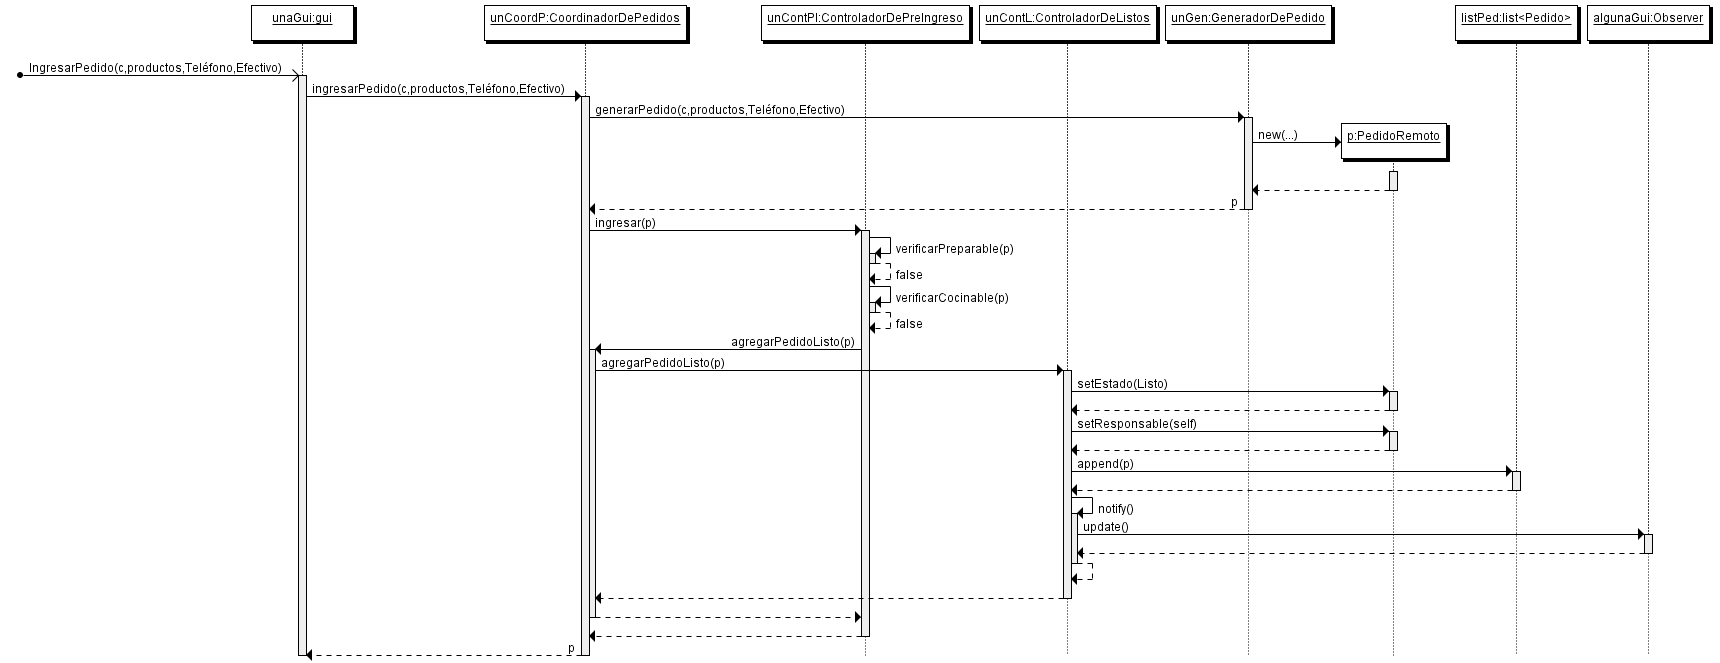
\includegraphics[height=21cm]{./figuras/remotoBebidas.png}
\caption{Ingreso de un pedido remoto de solo bebidas}
\end{figure}

El verifcarPreprable y su analogo para cocinable, basicamente recorren los productos del pedido, buscando si alguno tiene un tipo preparable o cocinable.

\begin{figure}[H]
\centering
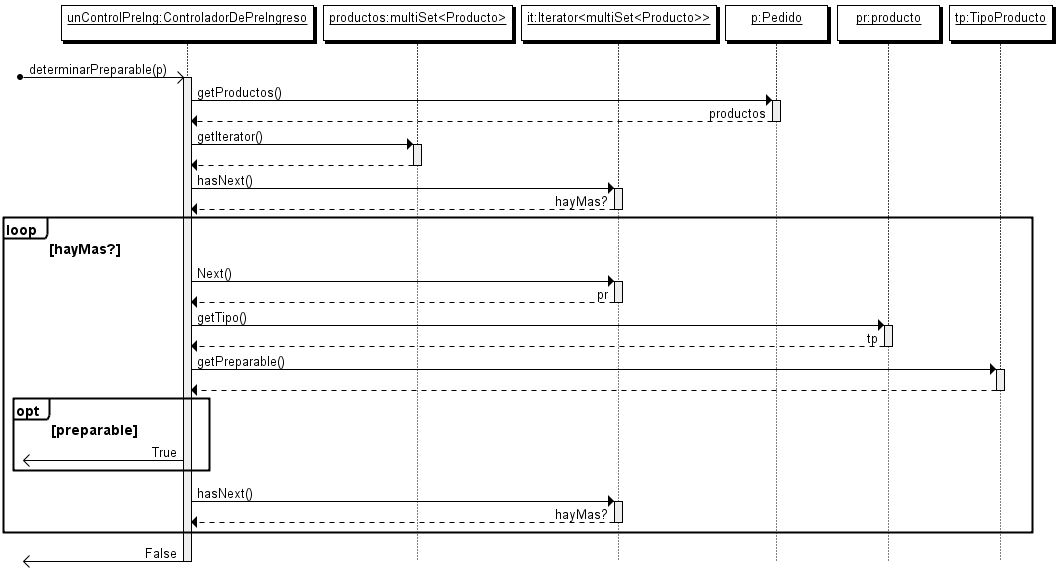
\includegraphics[height=9cm]{./figuras/determinarPreparable.png}
\caption{VerificarPreparable}
\end{figure}

\begin{figure}[H]
\centering
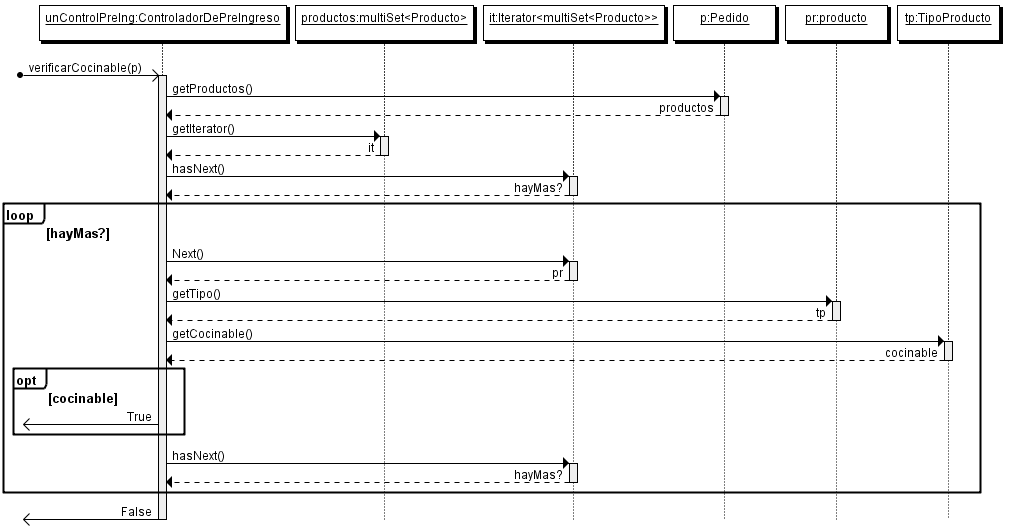
\includegraphics[height=9cm]{./figuras/determinarCocinable.png}
\caption{VerificarCocinable}
\end{figure}
%FIXME: o tocamos la imagen con el inkscape o justifamos las cosas que son de notacion rara

\subsubsection{Ingreso de un pedido con comidas}
De forma analoga al escenario anterior, supongamos que se va a ingresar un pedido, pero en este caso, el pedido si ten�a comidas, por lo que el controlador de pre ingresos se lo va a mandar al de ingresos. Este intenta pasarlo a la cocina para ver si esta puede hacerse cargo del pedido. Esto es asi porque en la especificaci�n se pide que si entra un pedido y el maestro estaba ocioso, se le notifique que prepare el pedido ingresado. Como conocer si los maestros estan preparando algo, no es asunto de este controlador lo que decidimos es que lo pase hacia la cocina y espere respuesta de esta. Modelaremos los dos escenarios, primero el caso en el que la cocina le dice que no puede hacerse cargo y en segundo lugar el caso en el que la cocina si acepta el pedido.

En el primer caso, el controlador de ingresos se hace cargo del pedido, cambiando su estado, marcando el pedido como ingresado y agregandolo a la cola.

\begin{figure}[H]
\centering
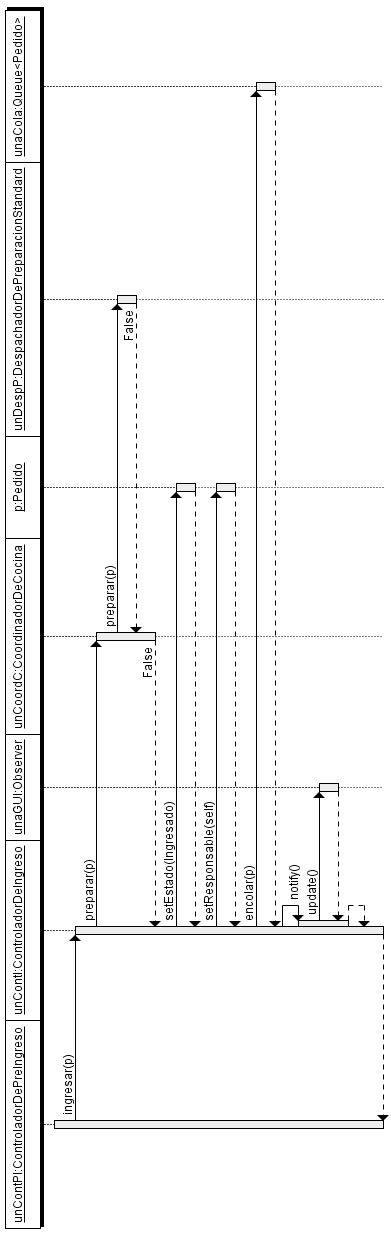
\includegraphics[height=6cm]{./figuras/remotoComidas.png}
\caption{Ingreso de un pedido remoto con comida que queda encolado para su ingreso}
\end{figure}

En el segundo caso, como se va a hacer cargo la cocina, el controlador de ingreso no debe hacer nada cuando se regresa la llamada.

\begin{figure}[H]
\centering
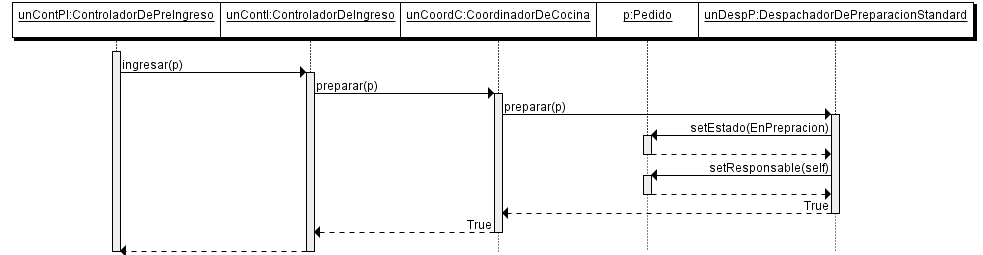
\includegraphics[height=4cm]{./figuras/remotoComidasquedapreparando.png}
\caption{Ingreso de un pedido remoto con comida que pasa a estar preparando}
\end{figure}

\subsubsection{Despacho de un pedido}
Cuando el pedido esta cocinado es responsabilidad de el controlador de listos. Una vez que el pedido esta listo, se puede despachar. Despachar tiene una semantica diferente segun el origen del pedido, por eso es que el controlador posse un despachar para los subtipos remotos, otro para el pedido de mesa y finalmente un tercer despachar para pedidos de mostrador.

En el escenario en el cual el pedido a despachar es de origen remoto, el controlador de listos, lo que hace es sacarlo de la lista, marcarlo como que salio en entrega y avisar de esto al coordinadorDePedido para que avise al controlador de entrega. Ademas notifica a su observador del evento. Esto se hace con la intenci�n de que la gui se entere de que un pedido salio de esta lista y la refresque.

El controlador de entregas pone al pedido en su lista de pedidos, y se asigna como responsable de la cancelaci�n del mismo.

Veamos el diagrama de secuencia comenzando la misma con la llegada de un mensaje de despachar al coordinador de pedidos

\begin{figure}[H]
\centering
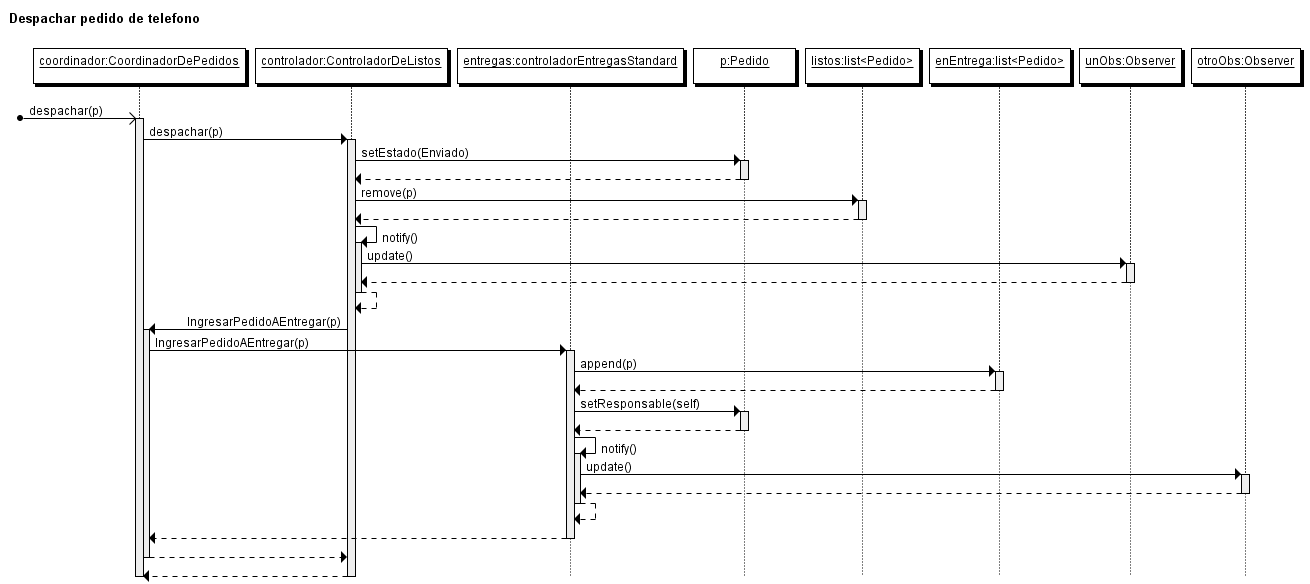
\includegraphics[height=7cm]{./figuras/despacharPedidoTelefono.png}
\caption{Despacho de un pedido telefonico}
\end{figure}

Otro escenario diferente lo constituye el despacho de un pedido de mesa. En este caso, el pedido deja la orbita del controlador de lista, para pasar al controlador de pedidos de mesa, el cual se encargara cuando se cierre la misma de asignar la forma de pago a los pedidos. Este encargado tambi�n se hace cargo de la cancelaci�n. Ambos controladores ademas notifican a su observador de los cambios en su lista.

El diagrama de secuencia es el siguiente:

\begin{figure}[H]
\centering
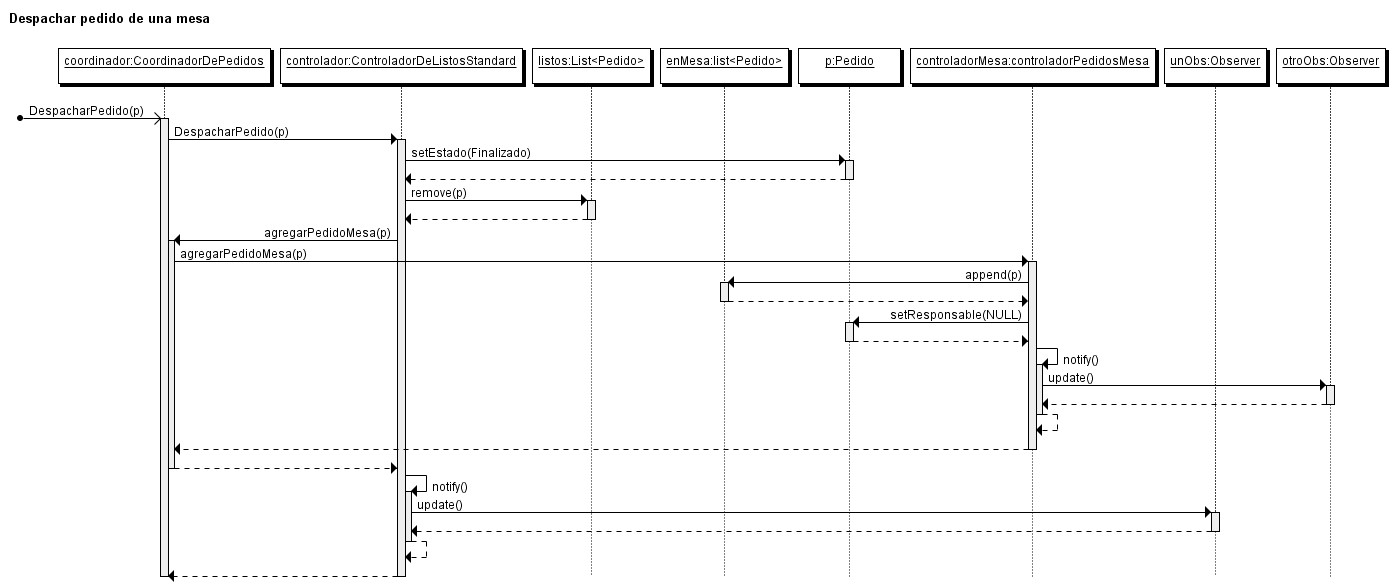
\includegraphics[height=7cm]{./figuras/despacharPedidoMesa.png}
\caption{Despacho de un pedido de mesa}
\end{figure}

Finalmente en el caso de un pedido de mostrador, el controlador de listos solo lo marca como terminado, ya que el pedido fue entregado y se conoce su forma de pago. Por lo tanto la secuencia es la siguiente:

\begin{figure}[H]
\centering
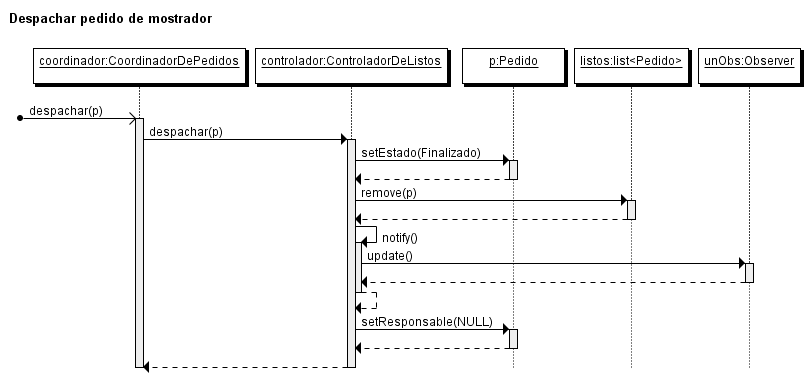
\includegraphics[height=8cm]{./figuras/despacharPedidoMostrador.png}
\caption{Despacho de un pedido de mostrador}
\end{figure}

\subsubsection{Pedido de proximo pedido a preparar}
Cuando el maestro termina de preparar un pedido (o sub pedido) se notifica al sistema. Entonces el despachador se encargado de pedirle al coordinador de la cocina que le consiga un pedido. Este habla con el controlador de ingreso para pedirle el pedido. Modelaremos el escenario en el cual el coordinador pide un pedido al controlador de ingreso. 

Para solicitar un pedido, se suministra al controlador de ingreso un TipoProducto, que le permite realizar la busqueda del primer pedido en la cola que contenga dicho tipo de producto. Esto es util si en un futuro se extienden los tipos de productos, o por ejemplo un maestro pasa a ser capaz de preparar otras cosas.

El controlador de ingreso entonces se encarga de buscar si en su cola hay alguien que cumpla tener algun producto del tipo solicitado. Si lo encuentra lo devuelve, sino devuelve NULL para informar que no tiene ningun pedido que contenga ese producto, por lo que el controlador quedara ocioso.

En el caso de tener que sacar un pedido de la cola, el controlador de listos hace un notify para invocar el update de su observador, por ejemplo para que se redibuje la cola de ingreso.

\begin{figure}[H]
\centering
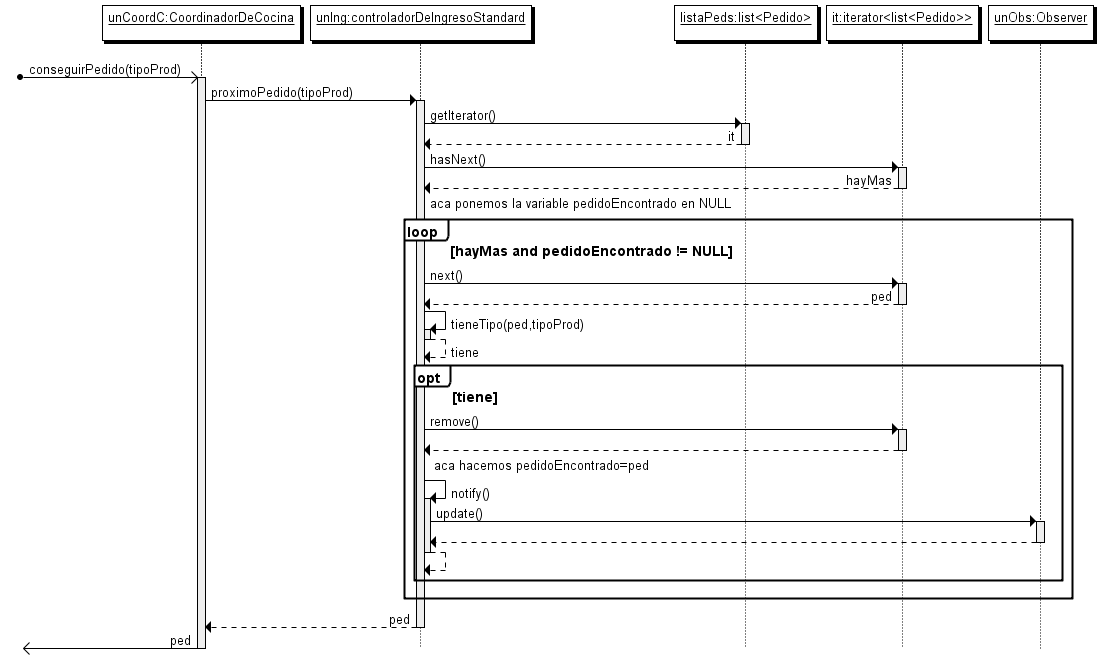
\includegraphics[height=8cm]{./figuras/proximoPedido.png}
\caption{Seleccion del proximo pedido}
\end{figure}

tieneTipo se encarga de recorrer los productos del pedido para ver si hay alguno con un cierto tipo de producto, el siguiente diagrama permite modelar la secuencia desatada por la ejecuci�n de este metodo.

\begin{figure}[H]
\centering
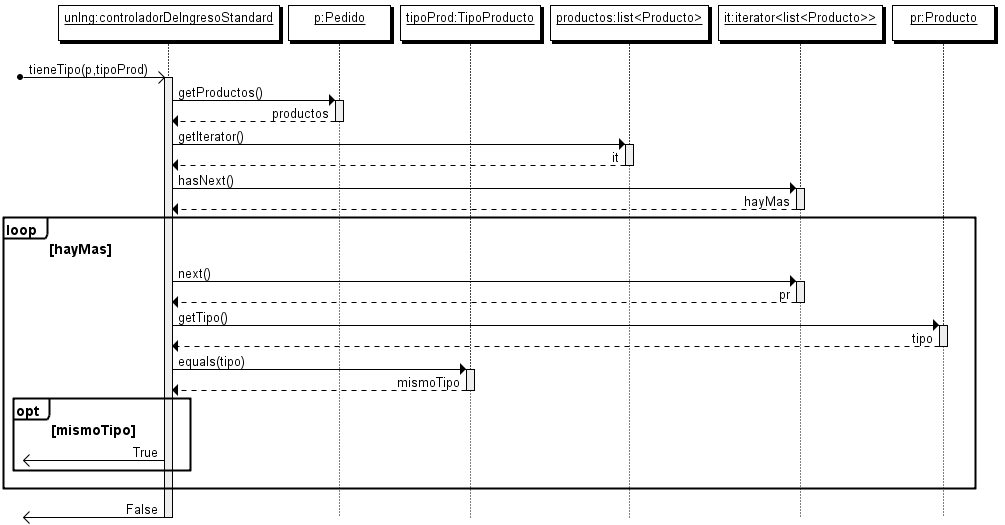
\includegraphics[height=8cm]{./figuras/tieneTipo.png}
\caption{tieneTipo}
\end{figure}

%TODO: decidir aridad de esta funci�n
%TODO: mostrar pseudocodigo

\subsubsection{Notificaci�n de entrega}
Cuando el usuario notifica una entrega, selecciona el pedido de la lista de pedidos con entrega pendiente e indica que fue entregado. Al hacerlo, se notifica al coordinador de pedidos, que pasa la llamada al controlador de entregas. El mismo busca el pedido que debe marcar como finalizado, lo marca y setea en \verb0NULL0 el encargado de cancelaci�n, ya que el pedido no puede ser cancelado a partir de este momento. Luego notifica a su observador que un pedido salio de su cola, por ejemplo para que la GUI que muestra los pedidos con entrega pendiente se refresque.

El escenario donde se notifica la entrega de un pedido, puede modelarse con el siguiente diagrama de secuencia:

\begin{figure}[H]
\centering
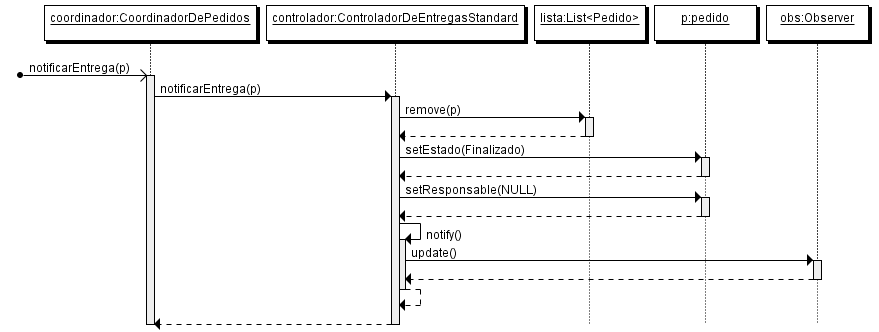
\includegraphics[height=7cm]{./figuras/notificarEntrega.png}
\caption{Notificacion de pedido entregado}
\end{figure}


\subsubsection{Cerrado de mesa}
Para cerrar una mesa el usuario ingresa el numero de mesa que desea cerrar, elegiendo tambi�n la forma de pago. La GUI pasa el mensaje al coordinador de pedidos, el cual propaga la llamada hacia el controlador de mesa, que se va a encargar de completar la forma de pago de los pedidos de la mesa seg�n el parametro pasado y los quita de la lista de pedidos con entrega pendiente. Entonces notifica a su observador de que se modific� su lista de pedidos.

El siguiente diagrama nos permite modelar dicho escenario:

\begin{figure}[H]
\centering
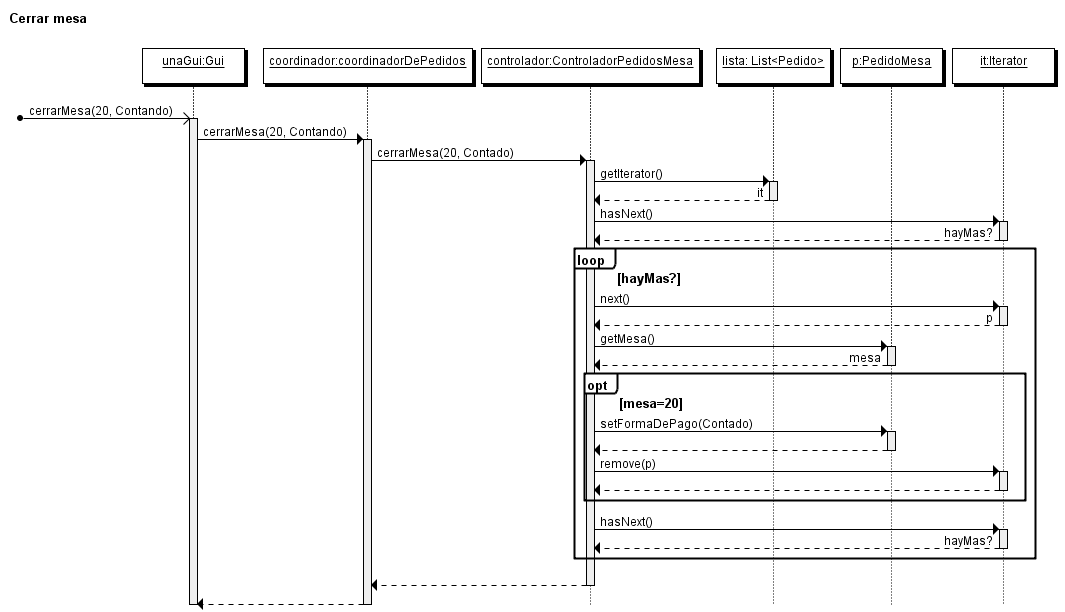
\includegraphics[height=9cm]{./figuras/cerrarMesa.png}
\caption{Cerrado de mesa}
\end{figure}

\subsubsection{Consulta de estado}
Dado que la GUI sabe mostrar pedidos, este escenario queda bastante simple, ya que la interfaz lista los pedidos, permitiendo al encargado filtrar o buscar por ejemplo por cliente o ID. Una vez que el encargado selecciona un pedido, solicita ver el estado y se llama al getEstado del pedido.

\begin{figure}[H]
\centering
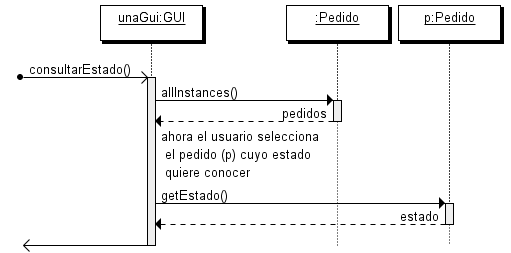
\includegraphics[height=9cm]{./figuras/consultarEstado}
\caption{Notificacion de pedido entregado}
\end{figure}

\subsubsection{Mover un pedido en la cola de ingreso}
Para mover un pedido en la cola de ingreso, la GUI se encarga de pedir la lista de pedidos en ingreso, la muestra y luego el encargado selecciona un pedido y puede elegir entre subir o bajar.

A continuaci�on mostramos un escenario en la que se pide subir un pedido en la cola. Vamos a suponer que el pedido a subir no es el primero, de esta manera nos evitamos usar un alt.

El controlador de pedidos pasa las llamadas al controlador de ingreso, que se encarga de obtener el indice del pedido, sacarlo y volverlo a poner en la posicion inmediatamente superio a la que tenia antes.

\begin{figure}[H]
\centering
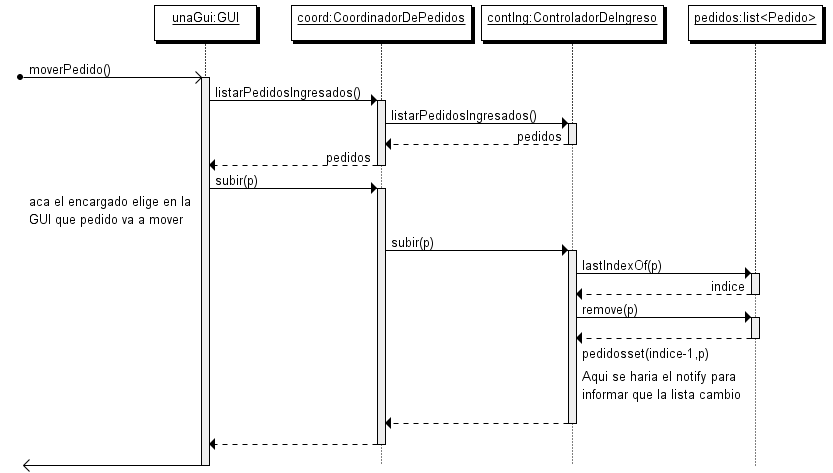
\includegraphics[height=10cm]{./figuras/subirPedido.png}
\caption{Subir un pedido en la cola de ingreso}
\end{figure}


\section{Creaci�n y registro de pedidos}
En este componente se agrupan las clases que entran en juego al momento de crear un nuevo pedido.

La clase GeneradorDePedidos sirve de punto de entrada a este componente. El mismo posee el m�todo generarPedido, que es invocado por el Coordinador de pedidos, a fin de que se ingrese al sistema un nuevo pedido.

El Generador se encarga de llamar al controladorDeStock para que verifique que el stock existente sea capaz de satisfacer al pedido. Ademas el generador realiza el decremento del stock, y se encarga de realizar el callback a la gui en caso de que un insumo quede por debajo de su stock critico. %TODO: callback como?
El controlador de stock no es una clase abstracta porque creemos que no es probable que cambie su funcionamiento, el cual es bastante concreo, es decir revisar los elementos necesarios para armar los productos propios de un pedido y decrementar el stock. 

Luego de que se regisr� el decremento de stock, el Generador se encarga de llamar al EstimadorDeTiempos. Esta clase es abstracta, ya que pensamos que como la pizzeria desea ir refinando estas estimaciones, es probable que la forma de estimar se modifique de forma periodica. Por lo tanto, decidimos aplicar el \textit{Strategy pattern} a fin de poder lograr varias estrategias de estimaci�n. La Estimaci�n desarrollada en \ref{modifEstim} es implementada por la clase EstimadorBasico.

\textcolor{Red}{TODO: interacciones de estas clases con la GUI}

\textcolor{Red}{TODO: explicacion de metodos importantes}
\subsection{Modelado de escenarios}

\subsubsection{Creacion de un pedido}
Cuando el coordinador de pedidos recibe la orden de crear un nuevo pedido, la deriva al generador de pedidos. Este se encargar� de devolverle un pedido nuevo. El generador de pedidos invoca al controlador del stock, para que verifique la factibilidad de ingresar el pedido, en caso de no ser posible el generador producira una excepcion que sera propagada para porder mostrar que producto no pudo satisfacerse.

En este escenario modelaremos el proceso de creaci�n de una forma general, en particular para un pedido de mostrador, para luego mostrar escenarios particulares que pueden ocurrir durante este proceso.

En primer lugar el generador invoca al controlador de stock para que realice el chequeo y en caso de ser posible decremente el sotck. 

Luego se genera un ID para el pedido y se lo crea. Una vez creado el pedido, este pasa al asignador de horno que establece que horno le corresponde al pedido (en caso de que corresponda). Luego se procede a realizar la estimaci�n de tiempos de cocci�n. Finalmente el pedido queda ingresado

El diagrama de secuencias es el siguiente:

\begin{figure}[H]
\centering
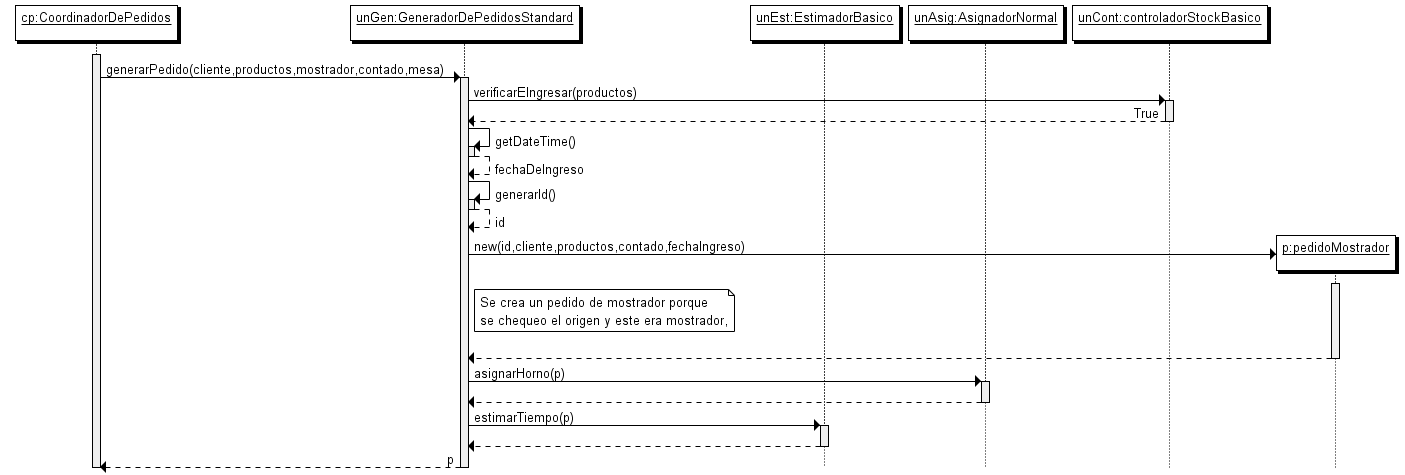
\includegraphics[height=9cm]{./figuras/crearMostrador.png}
\caption{Creaci�n de un nuevo pedido}
\end{figure}

\subsubsection{Estimacion de tiempos}

\subsubsection{Verificaci�n de stock}
El verificador de stock tiene por responsabilidad controlar que solo ingresen pedidos que puedan ser satisfechos. Ademas en caso de ser necesario debera notificar la existencia de insumos en stock critico.

Como vimos en el escenario anterior, el generador invoca el metodo verificarEIngresar. Este metodo va a intentar decrementar el stock de los insumos de cada producto del pedido que se desea armar. Para eso va a decrementar el stock siempre que sea posible, guardando aquellos productos cuyos insumos ya modifico para poder hacer rollback en caso de que el pedido no se pueda satisfacer. Si ocurre que hay un insumo de un producto cuyo insumo es insuficiente, se procede a restablecer el stock ya decrementado y luego se genera un excepcion que permite que se pueda mostrar en pantalla cual fue el pedido que genero el error al intentar ingresar.

En cambio si todos los productos se pudieron ingresar, la funci�n retorna True para indicar que termino exitosamente.

\begin{figure}[H]
\centering
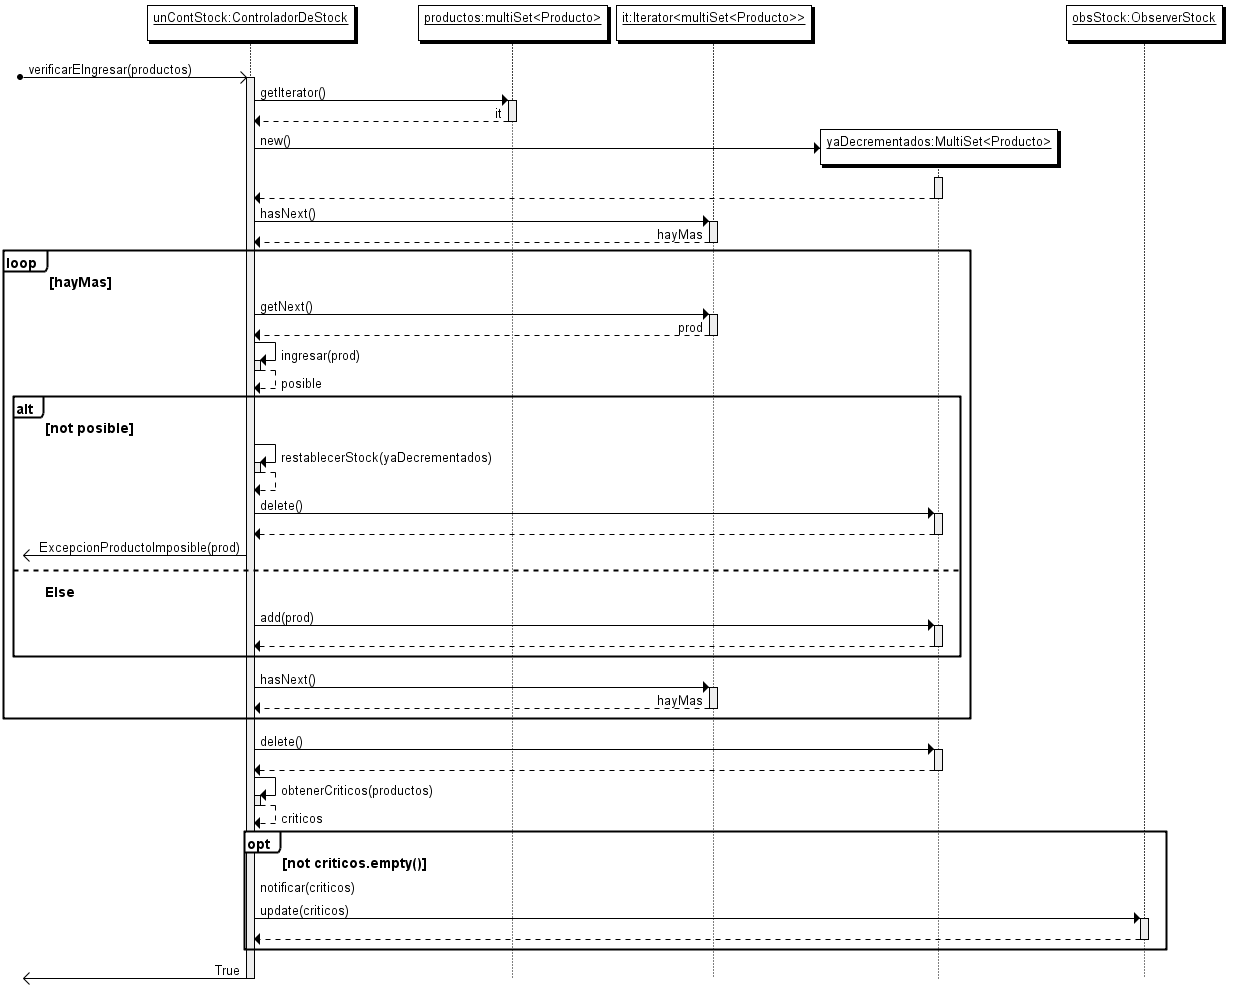
\includegraphics[height=15cm]{./figuras/verificarEIngresar.png}
\caption{Verificaci�n y decremento de stock de los insumos}
\end{figure}

Decidimos factorizar el diagrama de modo que algunas interacciones las mostraremos a continuaci�n. El metodo ingresar realiza la verificaci�n pero a nivel de cada producto, es decir revisa dado un producto que exista una cantidad de insumos necesaria. Al igual que el metodo anterior va recordando los stocks que ya modifico para hacer rollback en caso de que sea necesario.

\begin{figure}[H]
\centering
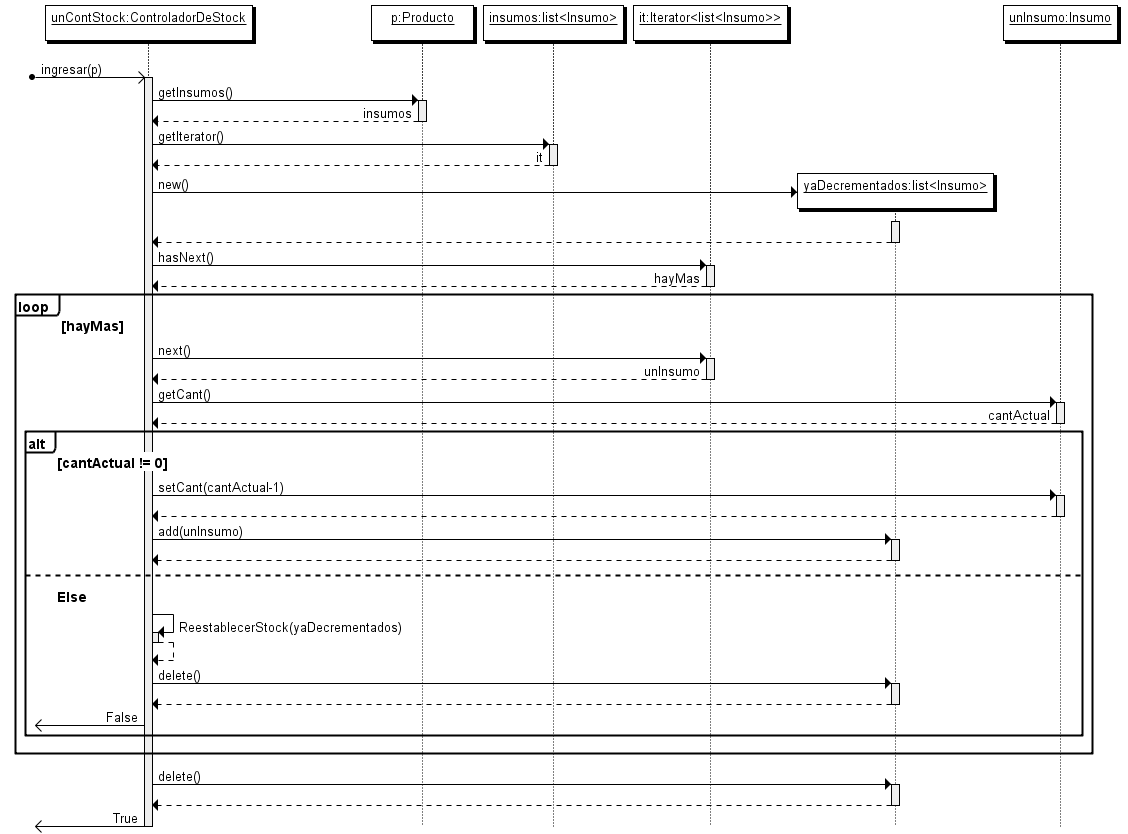
\includegraphics[height=11cm]{./figuras/ingresar(ControladorStock)}
\caption{Verificaci�n y decremento de stock de los insumos}
\end{figure}

Hay dos metodos restablecerStock, uno trabaja sobre productos y otro a nivel de insumos. El primero recorre los productos llamando al segundo para los insumos de cada producto que itera. Mientras que a nivel de insumos, lo que se hace es incrementar la cantidad de cada insumo que aparece en la lista. Como dijimos anteriormente, estos metodos permiten realizar un rollback para dehacer los cambios hechos en el stock en el caso de que la operaci�n de ingreso no sea exitosa

\begin{figure}[H]
\centering
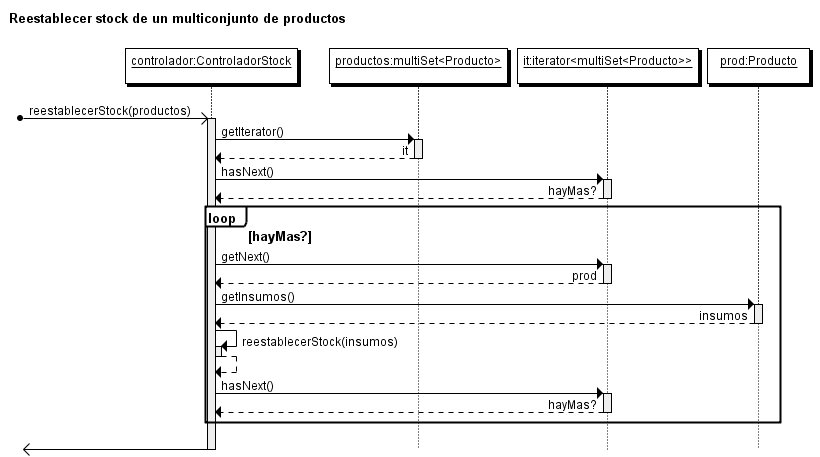
\includegraphics[height=9cm]{./figuras/reestablecerStockProductos}
\caption{restableciendo el stock de los productos cuyo }
\end{figure}

\begin{figure}[H]
\centering
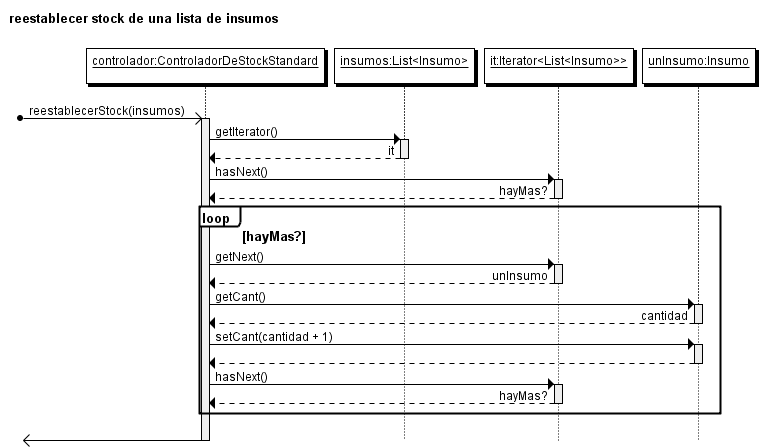
\includegraphics[height=9cm]{./figuras/reestablecerStockInsumos}
\caption{restableciendo el stock de los productos cuyo }
\end{figure}

{\color{purple}
\subsubsection{asignar horno}
\begin{itemize}
\item asignacion automatica
\item asignacion manual
\end{itemize}
}
\subsubsection{Estimacion de tiempos}

\textcolor{Red}{TODO: pseudocodigos que muestren algoritmos como por ej estimacion de tiempos}

\section{Gesti�n de clientes}
Este componente es el responsable de la gesti�n de los datos de clientes. Adem�s
de las funcionalidades b�sicas de ABM, este componente permite acciones tales
como validar clientes para realizar las operaciones que requieren de autenticaci�n.

Como se describiera en \ref{metodosEstaticos}, la clase Cliente tiene m�todos 
est�ticos as� como m�todos convencionales que permiten llevar a cabo las tareas
de ABM. Sin embargo, como tambi�n es necesaria la funcionalidad adicional de validaci�n
de usuarios, en este caso se implementa un objeto Controlador que es responsable de
llevar a cabo estas tareas. Esto se hace para respetar SRP.

Las implementaciones de los m�todos de estas clases son relativamente sencillas.
El Controlador realiza b�squedas en el conjunto de instancias para chequear los
datos requeridos por la interfaz, y responde en funci�n de los mismos. En principio
no parecen ser necesarios algoritmos sofisticados de b�squeda, pero eventualmente
se podr�a modificar la implementaci�n de dichos m�todos manteniendo su interfaz
para mejorar la eficiencia si se lo juzgara necesario. La encapsulaci�n que provee
el objeto hace que estos cambios no afecten al resto del sistema puesto que tanto
la signatura como la sem�ntica de los m�todos se mantendr� intacta.

\subsection{Modelado de escenarios}

% TODO: hacer algun DS, la verdad que no hay gran cosa para poner ac�
\textcolor{Red}{TODO: escenarios que muestren el comportamiento de estas clases en los fenomenos pedidos en el enunciado}


\section{Cocina}
La cocina es el componente de mayor complejidad del sistema. Al igual que en el manejo de pedidos fuera de la cocina, tenemos una clase que sirve de punto de entrada y de controlador de flujo dentro de la cocina, derivando a los pedidos al despachador o controlador correspondiente. Esta clase es la que tiene contacto con el controlador de ingresos, de modo que todo pedido que quiere entrar en la cocina pasa por este coordinador. Cuando recibe un pedido, o pide un pedido, esta clase es la que decide quien debe hacerse cargo de recibir al pedido. Si consideramos el funcionamiento actual de la pizzer�a, donde los pedidos que llegan a la cocina son preparables y cocinables, al ingresar un pedido a la cocina, el coordinador lo va a enviar al despachador de preparacion y luego cuando este lo termine se lo enviar� al despachador de cocci�n. 

El despachador de preparaci�n es una clase abstracta que tiene por responsabilidad mantener la cola de pedidos que deben ser preparados, conocer que subpedidos se prepararon y notifiar cuando el pedido ya fue preparado. Decidimos que sea abstracta porque es factible considerar que hay diferentes formas de manejar que pedido de los que estan esperando debe preparse a continuaci�n. Ademas, la implementaci�n de estas funcionalidades va a estar acoplada fuertemente con los tipos de productos existentes y el manejo que se le de a los mismos. Por ejemplo, es razonable que como la pizzer�a solo maneja pizzas y empanadas, las cuales son preparadas por un unico maestro, el despachador divida a un pedido en solo estas dos partes, sin embargo si en el futuro se agregan ensaladas, el pedido tendria que ser dividio de otra manera. Entonces a fin de dar mayor extensibilidad decidimos hacer que esta clase sea abstracta. En particular el despachador que se comporta como lo mostrado en la especificaci�n es implementado por DespachadorDePreparaci�nEstandard. Esta clase que hereda del despachador de preparaci�n, sabe distribuir pizzas y empanadas a sendos preparadores.

Preparador es una interfaz que tiene como metodo principal preparar. La idea es que este metodo sea el que hable con la gui para mostrar que se debe preparar. Decidimos hacer una interfaz para esto, porque si bien en este momento se muestra todo el contenido del pedido (o subpedido a preparar), esta estraetgia podr�a cambiar, si por ejemplo se desea tener un contro de cada producto del pedido. Entonces nuestro preparador especializado que implementa esta interfaz funciona como lo planteamos en la especificaci�n.

La clase despachadorDeHorno es la responsable del manejo de las colas de ingreso a los hornos, aplicando la politica correspondiente. En principio habiamos considerado que era conveniente separar la aplicaci�n de la politica del mantenimiento de las colas, sin embargo dado que la aplicaci�n de la politica requiere de un acceso completo a las colas, nos pareci� acertado acoplar ambas funcionalidades. La clase es abstracta, siguiendo el \textit{strategy pattern} a fin de permitir que se implementen diferentes politicas de manera flexible.

La clase ControladorHorno es una abstraccion de los modulos del horno, esta clase permite poner algo en un modulo, asi como tambi�n sacar algo de un modulo, o conocer que es lo que hay en cada modulo. Cada controladorHorno posee ademas un fraccionador que sabe fraccionar un pedido en partes que entran en un modulo, contando para eso con un diccionario que dado un tipo de pedido pueda decidir cuantos productos de ese tipo entran en cada modulo.

\textcolor{Red}{TODO: interacciones de estas clases con la GUI}

\textcolor{Red}{TODO: explicacion de metodos importantes}
\color{Blue}{
\subsection{Modelado de escenarios}
\subsubsection{Ingreso de pedidos a preparar}
En nuestra especificaci�n del sistema consideramos que el aviso de preparaci�n se produciria de manera automatica siempre que el maestro este ocioso y llegue un nuevo pedido. Tambi�n se produce de forma automatica cuando el maestro termina y hay algun pedido potencialmente preparable por el.

Es por esta raz�n que el ingreso de un nuevo pedido genera que se intente poner a preparar el pedido, ya que el controlador de ingreso no conoce el estado de los preparadores. El despachador de preparaci�n recibe estos pedidos y decide si puede derivarlos o no, en cuyo caso deben quedar encolados en el controlador de ingreso.

A continuaci�n modelaremos algunos escenarios que pueden producirse en estos casos. Para los escenarios utilizaremos los pedidos mixtos, ya que los pedidos simples son un caso particular de estos ultimos.

En el primer escenario, consideraremos que el pedido ingresa pero ambos maestros estan ocupados por lo cual el pedido debe encolarse en la cola de ingreso. 

El despachador estandar lo que hace es revisar si un pedido es asignable al maestro empanadero, para que esto ocurra el pedido tiene que contener alguna empanada y ademas el maestro empanadero debe estar libre. Si no, no se puede. En este escenario el maestro esta ocupado por lo que no se puede asignarle el pedido. La situaci�n del pizzero es similar, asi que tampoco se le puede asignar el pedido. Ergo, el mismo se rechaza.

\begin{figure}[H]
\centering
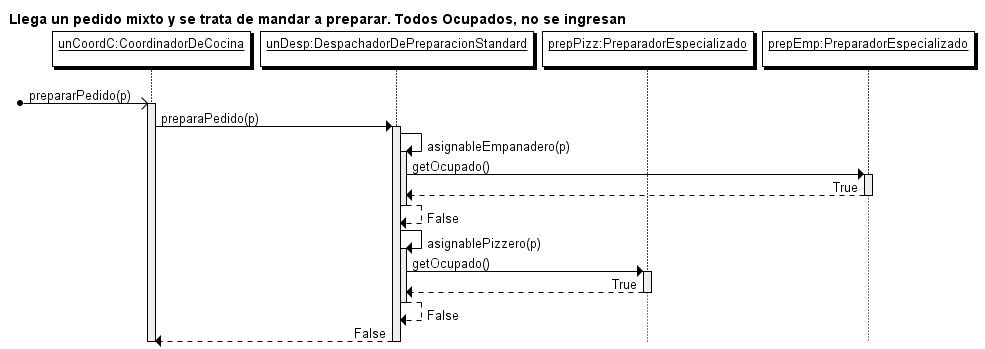
\includegraphics[height=6cm]{./figuras/mandanPrepararMixtoYEmpiezanNada.png}
\caption{Solicitud de preparacion de un pedido mixto cuando ambos maestros estan ocupados}
\end{figure}

Otro caso es aquel en el que uno de los maestros si esta dispuesto a comenzar la preparaci�n del pedido. En este caso, el pedido se encola para el empanadero (porque era mixto) pero comienza a preparse para el pizzero. Al hacerlo es necesario guardar alguna informaci�n sobre el pedido. Por ejemplo registrar que es mixto y que por lo tanto antes de estar listo se deben preparar los dos subpedidos (empanadas y pizzas). Y recordar que ese es el pedido que el pizzero esta preparando. Luego se entregan los subproductos a preparar al preparador y se notifica mediante el return que el pedido no debe quedar en la cola de ingreso, sino en preparaci�n.

\begin{figure}[H]
\centering
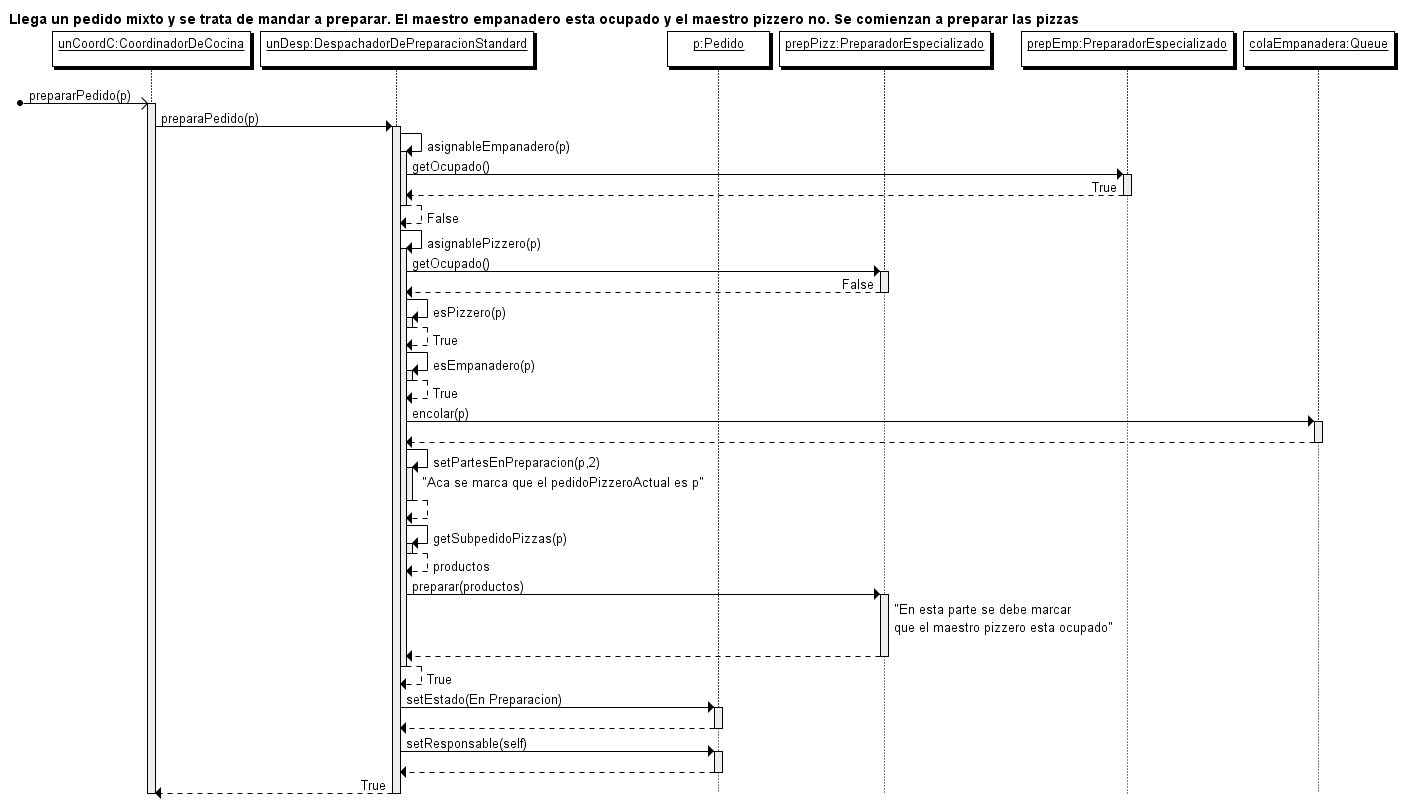
\includegraphics[height=10cm]{./figuras/mandanPrepararMixtoYEmpiezanPizzas.png}
\caption{Solicitud de preparacion de un pedido mixto cuando el maestro pizzero esta disponible}
\end{figure}

Finalmente podria ocurrir que ambos maestros esten ociosos, porque no habia ningun pedido en la pizzeria esperando por ser preparado. Y al llegar un nuevo pedido ambos comiencen a preparalo. La situaci�n es similar al caso anterior, pero en este caso no se encola el pedido, sino que se notifica a ambos preparadores para que estos luego realicen la notificaci�n.

\begin{figure}[H]
\centering
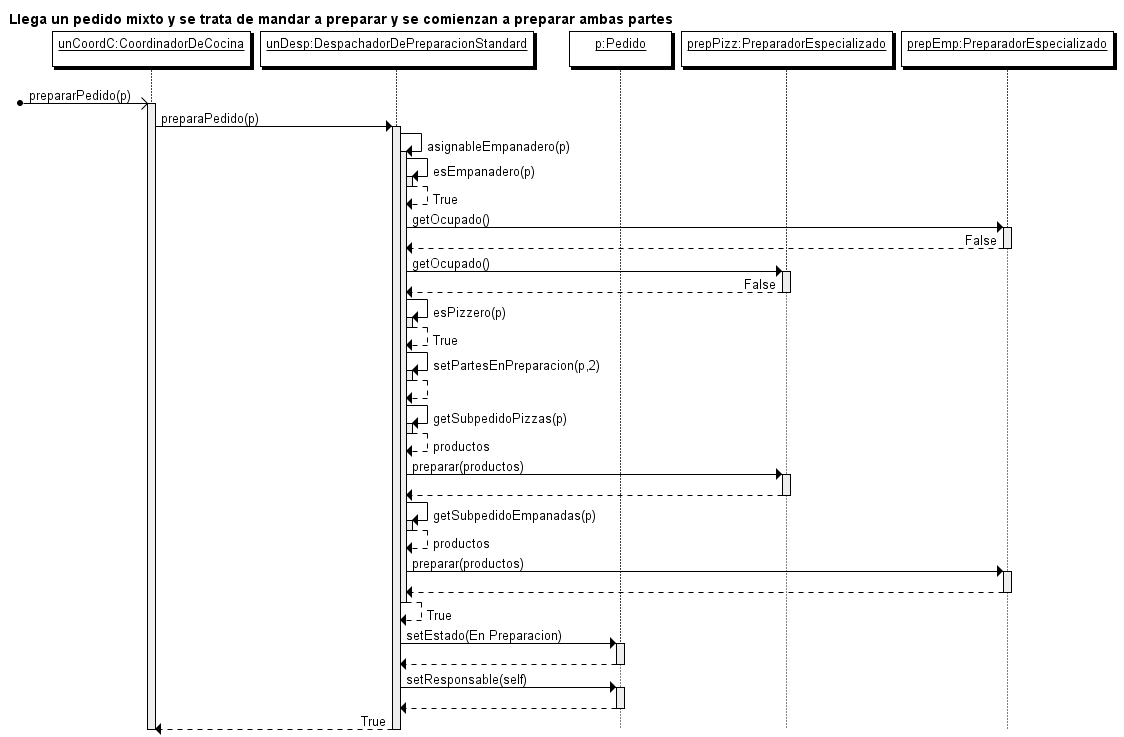
\includegraphics[height=11cm]{./figuras/mandanPrepararMixtoYEmpiezanAmbos.png}
\caption{Solicitud de preparacion de un pedido mixto cuando ambos maestros estan disponibles}
\end{figure}

\subsubsection{Terminancion de preparaci�n}


\subsubsection{Ingreso de pedidos al horno}
Luego de ser preparados los pedidos pasan a traves del coordinador de cocina hacia el despachador de coccion. Este despachador es quien se encarga de manejar las colas de los hornos segun alguna politica. En particular en este trabajo consideraremos la politica normal y la politica agil, las cuales fueron debidamente especificadas en el trabajo anterior.

Basicamente ambas politicas, o despachadores tienen una estructura interna similar. Se utiliza un diccionario de numero de modulo a pedido que lo ocupa, para cada horno, hay dos colas de pedidos, pueden ser listas, ya que se por ejemplo se busca dentro de ellas, un diccionario que permite saber que partes faltan cocinar de un pedido y finalmente una variable de estado (2 en el caso de la politica agil) que permiten conocer que pedido esta a mitad de coccion, con elementos sin cocinar, y elementos cocinados o dentro del horno (la politica agil necesita 2 de estas variables ya que puede haber un pedido grande y un pedido chico en esta condicion).


%TODO: tal vez este no es el lugar para tantos detalles
Luego de terminar la preparacion de un pedido, el despachador invoca al coordinador, el cual a su vez llama al despachador de cocci�n. En un primer escenario a considerar, el pedido llega al despachador y como no hay lugar para entrar a su horno, se lo encola. Antes de encolarlo, se invoca al fraccionador, correspondiente al controlador del horno del pedido, para que separe al pedido en grupos de productos que se pueden colocar en un modulo. Es decir si el pedido es 3 pizzas y 3 empanadas y entran 2 empanadas por modulo y una pizza por modulo, una posible separacion de los productos del pedido es \{ 1 pizza, 1 pizza, 1 pizza, 2 empanadas, 1 empanada \}

En este escenario se asume que el horno 1 es el asignado al pedido.

%TODO: colocar el pseudocodigo del despachador

El diagrama de secuencia resultante es el siguiente:

\begin{figure}[H]
\centering
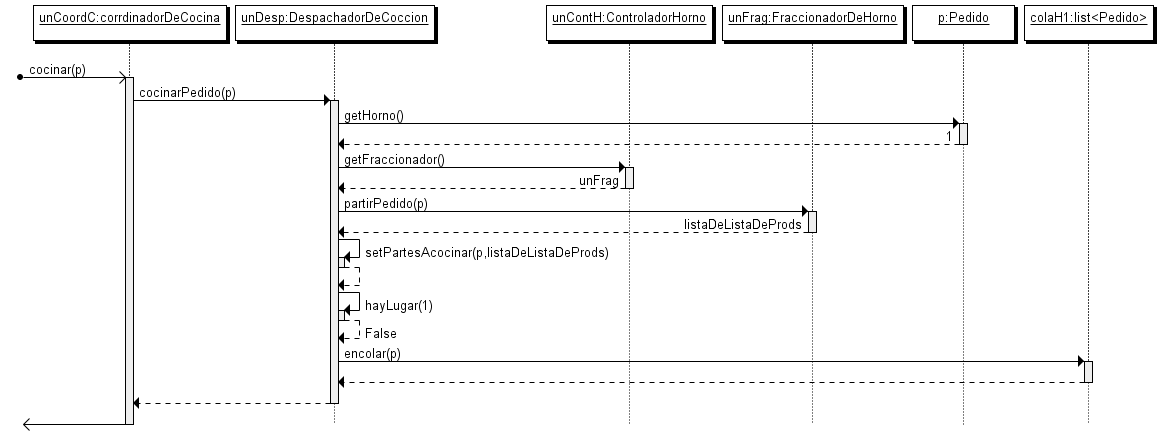
\includegraphics[height=6cm]{./figuras/llegaCocinarYseEncola.png}
\end{figure}

Otro escenario a considerar, comienza de igual manera que el anterior, pero esta vez si hay lugar en el horno para que el pedido entre. Lo que se hace es meter una parte del pedido en algun modulo libre, esto se repite mientras queden modulos libres o se termine el pedido. Por simplicidad en este escenario consideramos el caso donde solo habia un modulo libre. Una vez hecho eso, lo que ocurre es que se actualiza el estado interno. Por eso en este diagrama, al igual que en el anterior hay muchos automensajes, los cuales se deben a la gran cantidad de informaci�n interna que se necesita para mantener las politicas de acceso a los hornos.

\begin{figure}[H]
\centering
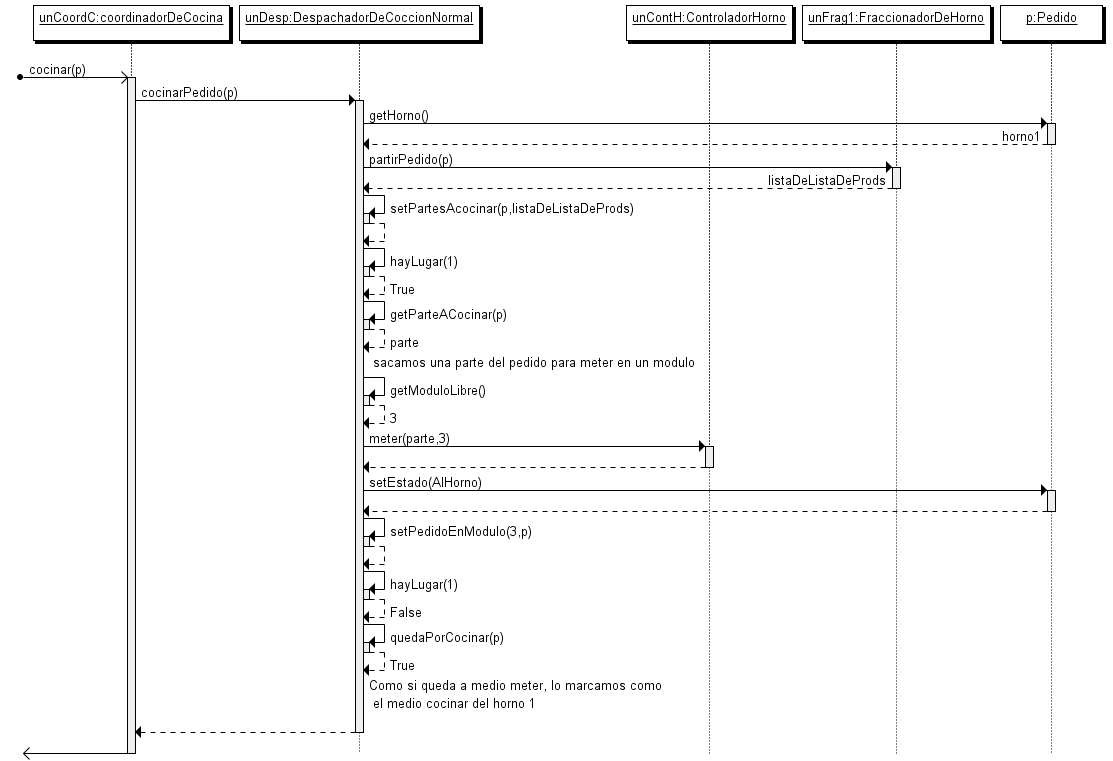
\includegraphics[height=6cm]{./figuras/llegaCocinarYNoseEncola.png}
\end{figure}

Queremos notar que estos escenarios aplican tambi�n para la politica agil, ya que los pedidos que llegan pueden quedarse encolados si no hay lugar (independientemente de si son agiles o no) y por otro lado pueden entrar si hay lugar libre, pero si hay lugar libre entran porque la cola es en esencia \textit{FIFO} en estas circunstancias, es decir si hay lugar vacio y solo hay un pedido, como se busca maximizar el uso del horno, se ingresa al mismo mas alla de su condicion de chico o grande. Nada impide que mas adelante se implemente una nueva politica que trate de hacer por ejemplo mas corto primero con conocimiento futuro, de modo que, por ejemplo use una cierta probabilidad $p$ para decidir si pone al pedido recien llegado al horno o no.

\subsubsection{Fin de coccion de una parte}
%FIXME: diagramas obsoletos porq cambio el md
Hasta ahora solo consideramos cuando los pedidos entran al despachador provenientes de la etapa de prepraci�n. Consideremos entonces que ocurre cuando se notifica la terminaci�n de la cocci�n de una parte que estaba en el horno.

Supongamos una politica normal, y que la parte del pedido que sale no es lo ultimo que quedaba por cocinarse. Para determinar si un pedido se termino de cocinar, se pregunta si queda alguna parte por cocinar y si hay alguna en el horno, si ambas respuestas son negativas, se termino de cocinar. Notar que no se esta intentando saber que partes fueron cocinadas, sino cuantas faltan. Otra nueva politica podria interesarse en tener un control mas estricto, por ejemplo para informar de forma mas precisa el estado de un pedido que es al horno.

La notificaci�n de que una parte se termino de preparar la recibe el controlador de horno, el cual recibe que modulo se liber�. El controlador pasa el mensaje al despachador, el cual actualiza su estado en funci�n de este evento y busca si puede poner a cocinar algo.

Lo que hace el despachador normal es buscar si hay un pedido a medio cocinar, es decir con partes sin cocinar y fuera del horno. Si hay uno se toma una parte de ese. Podria ocurrir que al pedido a medio cocinar solo le quedaba esa parte por cocinar, en cuyo caso ahora no hay ningun pedido a medio cocinarse en ese horno.�

Si no habia ninguno a medio preparar toma el proximo pedido de la cola y busca alguna de sus partes para enviar al controlador de horno. Este nuevo pedido podr�a pasar a ser el nuevo pedido a medio cocinar.

Si no habia ningun pedido en la cola tampoco, no tiene nada que hacer luego de actualizar su estado.

\begin{figure}[H]
\centering
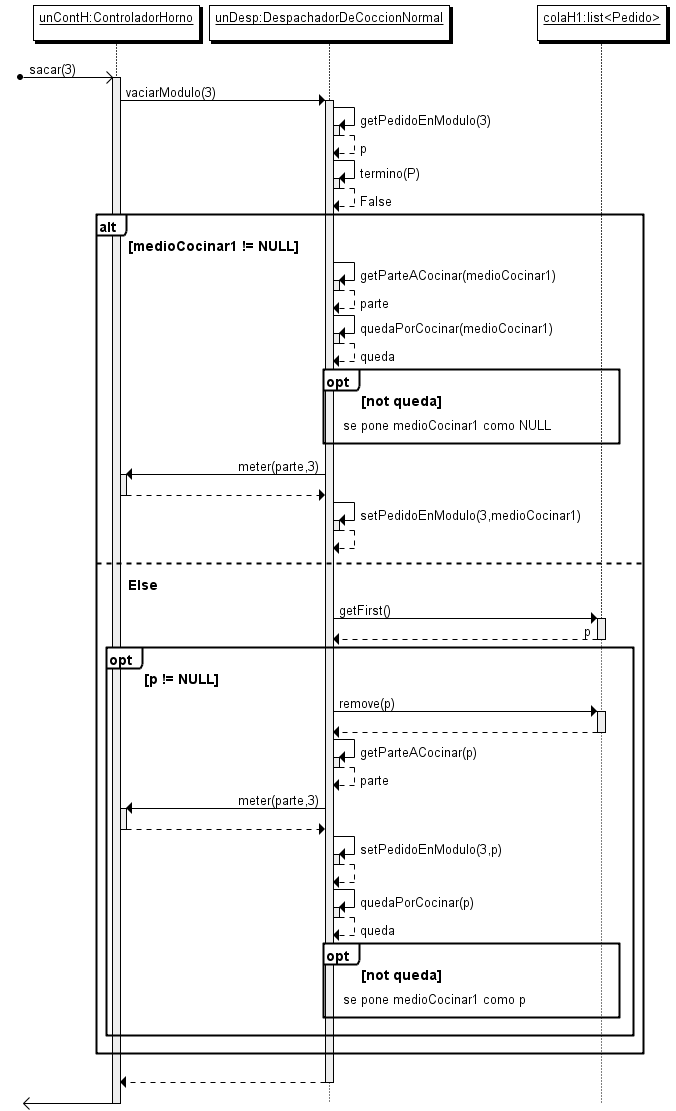
\includegraphics[height=18cm]{./figuras/saleUnPedidoNormalNoTermina.png}
\end{figure}

En el escenario donde la politica es agil, la situaci�n es similar, en particular en el caso de que el modulo que se vacia no es agil, es el mismo procedimiento. Si el modulo que se vacia si es agil, el funcionamiento se modifica. En vez de intentar meter el pedido a medio cocinar se busca el pedido chico a medio cocinar. Si no hay, lo que se hace es buscar si hay algun chico en la cola, cuando lo encuentra el proceso es similar al escenario anterior, solo que este pedido puede llegar a ser el chico a medio cocinar. Si tampoco lo encuentra, busca como si fuera una politica normal. Esto nos permite ver como la politica agil, frente a la ausencia de pedidos chicos, es exactamente igual a la politica normal.

\begin{figure}[H]
\centering
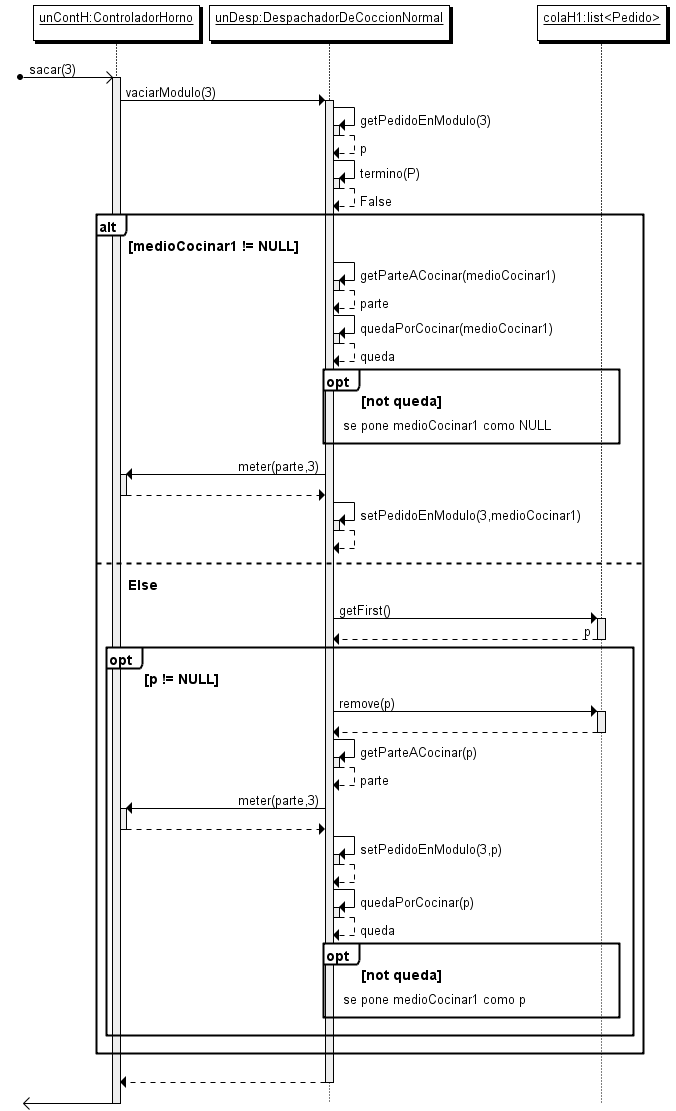
\includegraphics[height=18cm]{./figuras/saleUnPedidoNormalNoTermina.png}
\end{figure}

\subsubsection{Algo termina de cocionarse}

\textcolor{Red}{TODO: escenarios que muestren el comportamiento de estas clases en los fenomenos pedidos en el enunciado}

\textcolor{Red}{TODO: pseudocodigos que muestren algoritmos como por ej seleccion de proximo pedido a cocinar}


\section{Gesti�n de stock y productos}

Este componente se encarga de la gesti�n de los modelos correspondientes a
productos, tipos de procuto, insumos y las operaciones de alta y baja de los
mismos, as� como de las actualizaciones de sus valores.

Mediante la funcionalidad de ABM provista como se describe en \ref{metodosEstaticos}
es posible realizar los cambios necesarios al stock, tales como modificaciones de
precios o el ingreso de nuevos productos.

El Controlador de Stock es una entidad abstracta que se encarga de las modificaciones
de los valores de stock frente al ingreso o cancelaci�n de pedidos. Esta abstracci�n
se introduce para respetar DIP, y puesto que podr�a ser interesante brindar funcionalidad
m�s sofisticada en esta entidad. Por ejemplo, un controlador de stock m�s inteligente podr�a
realizar un seguimiento individual de todas las transacciones de stock llevadas a cabo
que permitir�a \textit{trackear} cada insumo.

El Controlador de Stock es responsable de emitir el evento de notificaci�n de stock
cr�tico, al que la GUI se suscribe para poder indicar al usuario que el stock requiere
de su atenci�n.

Las clases principales en lo que a modelos de datos respecta dentro de este componente
son Insumo y Producto. La clase TipoProducto permite reconocer cuando varios productos
tienen el mismo tipo y por tanto pueden tratarse de forma an�loga en cuanto a su
preparaci�n y cocci�n. 

El tipo de producto permite especificar adem�s si el producto es
cocinable o preparable. Si bien en el sistema actual los productos son ya sea preparable
y cocinables o ninguno de los dos, en el futuro la pizzer�a podr�a desear, por ejemplo,
comercializar ensaladas que solo requieren de preparaci�n y no de cocci�n. La existencia
de estos atributos permite flexibilidad adicional para extender la operatoria del
restaurante. Si bien esta elecci�n de atributos puede parecer limitante o arbitraria,
evaluamos que es factible categorizar de esta manera a cualquier tipo de producto
que podr�a venderse en una pizzer�a. Por lo tanto, no nos pareci� razonable agregar
complejidad al modelo agregando ``propiedades'' gen�ricas a los tipos de producto
(propiedades de las que \textit{cocinable} y \textit{preparable} ser�an un caso particular).

% TODO: hablar del repositorStock


\subsection{Modelado de escenarios}
% TODO: traer los diagramas de la parte de ingreso de pedidos

\textcolor{Red}{TODO: explicacion de metodos importantes}
% FIXME: vale la pena? creo que co los DS que estan en la parte de ingreso de pedidos alcanza y sobra


\section{Cancelaci�n}

La cancelaci�n de un pedido es un evento que puede producirse en cualquier momento de la
vida de un pedido hasta que pasa al estado finalizado. Como vimos en las secciones anteriores,
los pedidos pasan por los distintos componentes a lo largo de su estado de vida.

Para llevar a cabo una cancelaci�n, no es suficiente con cambiar el estado del pedido
a ``Cancelado'', sino que adem�s es necesario que el componente que est� manipulando
el pedido al momento de la cancelaci�n modifique su estado para reflejar este cambio.
Por ejemplo, un controlador de cola de horno debe retirar los elementos del pedido de las
colas correspondientes si se produce una cancelaci�n. Por esta raz�n, la cancelaci�n
afecta de alguna manera a todos los componentes del sistema, y es el �nico fen�meno
verdaderamente \textit{transcomponente} que debimos considerar.

Consideremos el esquema \ref{diag_componentes}, podemos ver en este diagrama como la cancelaci�n involucra a varios componentes. El siguiente esquema intenta mostrar esta idea:

\begin{figure}[H]
\centering
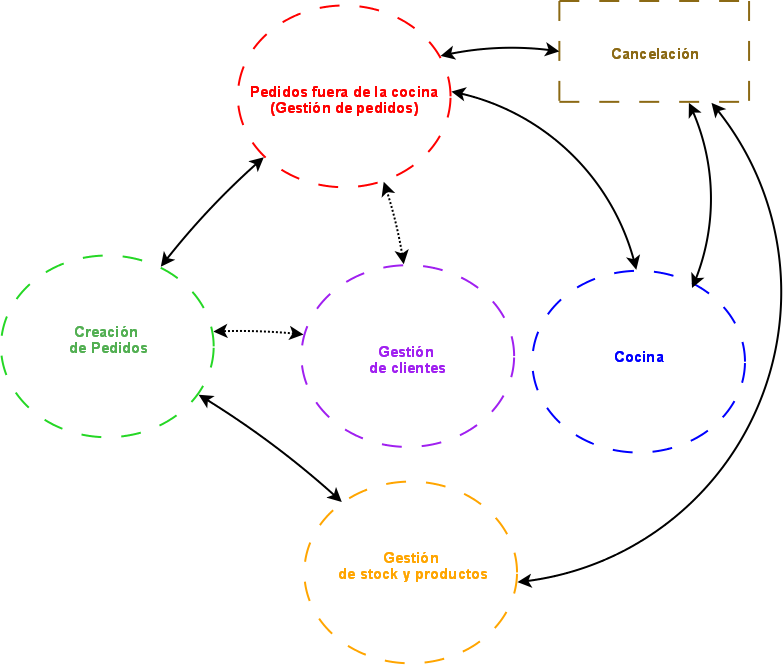
\includegraphics[height=10cm]{./figuras/conCancelacion.png}
\caption{Diagrama de componentes l�gicos con el evento de cancelaci�n}
\end{figure}

Es necesario presentar a la GUI una interfaz sencilla para permitir la cancelaci�n de un
pedido. En funci�n de esto, la GUI permite al usuario encontrar el pedido que desea cancelar
(utilizando alguno de los m�todos de b�squeda) y luego env�a un mensaje a una entidad id�nea
para realizar la tarea.
%FIXME: que onda con esto de los metodos de busqueda

En este punto nos encontramos con una dificultad particular: �Cu�l es esta entidad? Es claro
que no puede elegirse arbitrariamente alguno de los componentes del sistema puesto que no
es f�cil determinar cu�l de ellos est� ocup�ndose del pedido en un momento dado. Consideramos 
entonces varias opciones.

En primer lugar evaluamos agregar un m�todo \verb0cancelar(Pedido)0 en el CoordinadorDePedidos,
\textit{fa�ade} principal del sistema, que luego se encargue de determinar al componente
responsable de la cancelaci�n y le env�e la notificaci�n correspondiente. A su vez, para determinar
el responsable, consideramos dos estrategias:
\begin{itemize}
\item Propagar el mensaje desde el coordinador a todas las dem�s entidades, en una estrategia
      similar al \textit{flooding} en dispositivos de red. Esto tiene el problema de que no es
      limpio y no es f�cil determinar qu� fue lo que ocurri� con la cancelaci�n desde el
      coordinador.
\item Definir una entidad que sea capaz de, a partir de la informaci�n de un pedido, determinar
      qui�n es el responsable en ese momento y enviarle un mensaje. Esto tiene el problema de que
      est� fuertemente acoplado a la operatoria actual del sistema, y por lo tanto viola OCP
      ya que si se desean agregar nuevos tipos de pedido, ser� necesario modificar esta
      funcionalidad para que refleje las nuevas posibilidades. Para apegarse a SRP, esta funcionalidad
      ameritar�a un objeto nuevo, pero esto no evita el acoplamiento que se introduce y la
      disminuci�n de cohesi�n que se deriva.
\end{itemize}

Puesto que ninguna de estas opciones result� satisfactoria, investigamos un poco m�s
y finalmente elegimos una opci�n que se asemeja al patr�n \textit{Observer}. Apeg�ndonos
a ISP, definimos una interfaz que llamamos \textbf{Cancelador} y que indica que la 
entidad que la implementa es capaz de cancelar un pedido. Le asignamos a su vez a
cada pedido un \textbf{responsable}, que no es m�s que una clase que implementa
la interfaz Cancelador. Cuando un componente del sistema toma el control de un pedido,
se registra como responsable del mismo. Cuando el pedido reciba una cancelaci�n,
notificar� al responsable para que este lleve a cabo la cancelaci�n.

% TODO: si se van a pintar de algun color las clases que implementan Cancelador
% en el diagrama, aclararlo ac�.
Las clases que implementan la interfaz Cancelador (y por tanto pueden
hacerse responsables de un pedido) son:
\begin{itemize}
\item ControladorEntregas
\item ControladorIngreso
\item ControladorListos
\item DespachadorPreparacion
\item DespachadorDeCoccion
\item Preparador
\end{itemize}

Esta soluci�n es considerablemente limpia y permite f�cilmente extender el sistema
sin realizar modificaciones innecesarias. Veamos a continuaci�n algunos escenarios diferentes 
de cancelaci�n.

\subsection{Modelado de escenarios}
\subsubsection{Cancelaci�n de un pedido ingresado}

El primer escenario consiste en cancelar un pedido que estaba en la cola de 
ingreso. En este caso se debe sacar de dicha cola al pedido y se debe reestablecer 
el stock de los insumos que no se van a utilizar.

\begin{figure}[H]
\centering
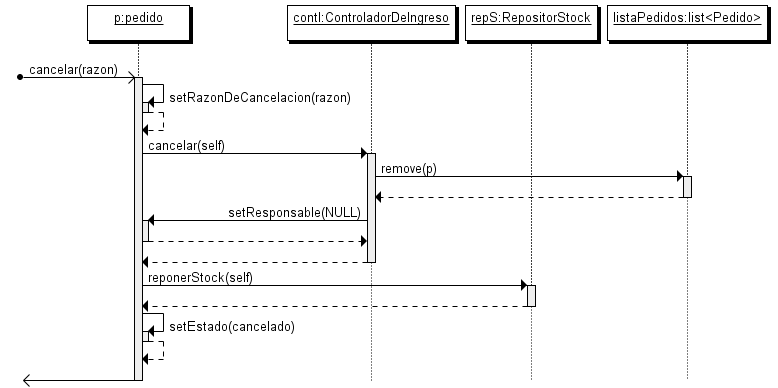
\includegraphics[height=8cm]{./figuras/cancelacionIngreso.png}
\caption{Cancelaci�n de un pedido ingresado}
\end{figure}

\subsubsection{Cancelaci�n de un pedido en preparaci�n}

En segundo lugar podemos considerar que ocurre cuando se cancela un pedido que 
estaba en preparaci�n. En este caso puede ocurrir que el pedido se estuviera 
preparando en el momento de su cancelaci�n, por lo que debe indicarse que se 
detenga la preparaci�n y que se indiquen qu� insumos se pueden reponer al stock.

Si la cancelaci�n se hace para un pedido que estaba en la cola nada m�s, el 
proceso es muy simple, solo se desencola esta parte que estaba en espera y se corrige
el estado del Pedido. A continuaci�n modelaremos un escenario m�s interesante, que corresponde
a la cancelaci�n de un pedido que ten�a sus empanadas siendo preparadas, asumiendo 
que hay otro pedido con empanadas en la cola esperando para ser preparados.

\begin{figure}[H]
\centering
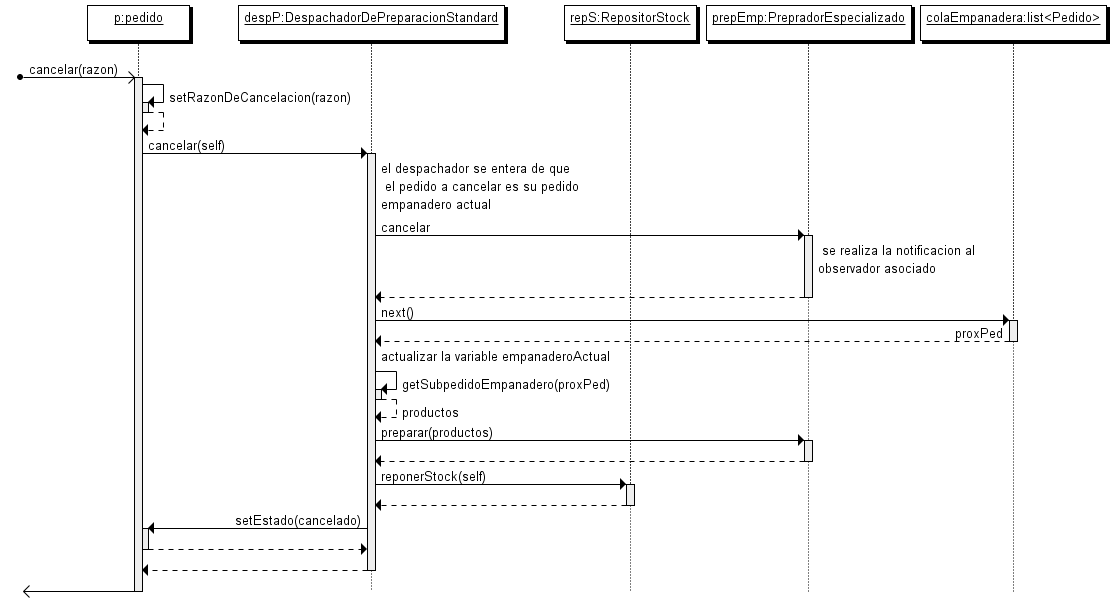
\includegraphics[height=11cm]{./figuras/cancelacionPreparacion.png}
\caption{Cancelaci�n de un pedido en preparaci�n}
\end{figure}

\subsubsection{Cancelaci�n de un pedido en cocci�n}

Otro lugar donde la cancelaci�n es conflictiva es durante la cocci�n de un pedido.
Si el mismo estaba en la cola del horno, el proceso es simple porque solo hay que 
sacarlo de la misma. Por otra parte, si el pedido estaba en el horno o estaba a medio cocinar, 
hay que avisar al maestro para que retire el pedido del horno y corregir el estado de los hornos.

Vamos a modelar el escenario en el que el pedido que se cancela era un pedido a medio 
cocinar del horno 1. Entonces, hay que avisar su cancelaci�n, y buscar un nuevo pedido 
para poner en su lugar. Vamos a suponer tambi�n que el pedido tenia dos partes en cocci�n, 
que no estaban en m�dulos �giles y que el pr�ximo pedido de la cola necesitaba de mas 
de 2 modulos para cocinarse.

\begin{figure}[H]
\centering
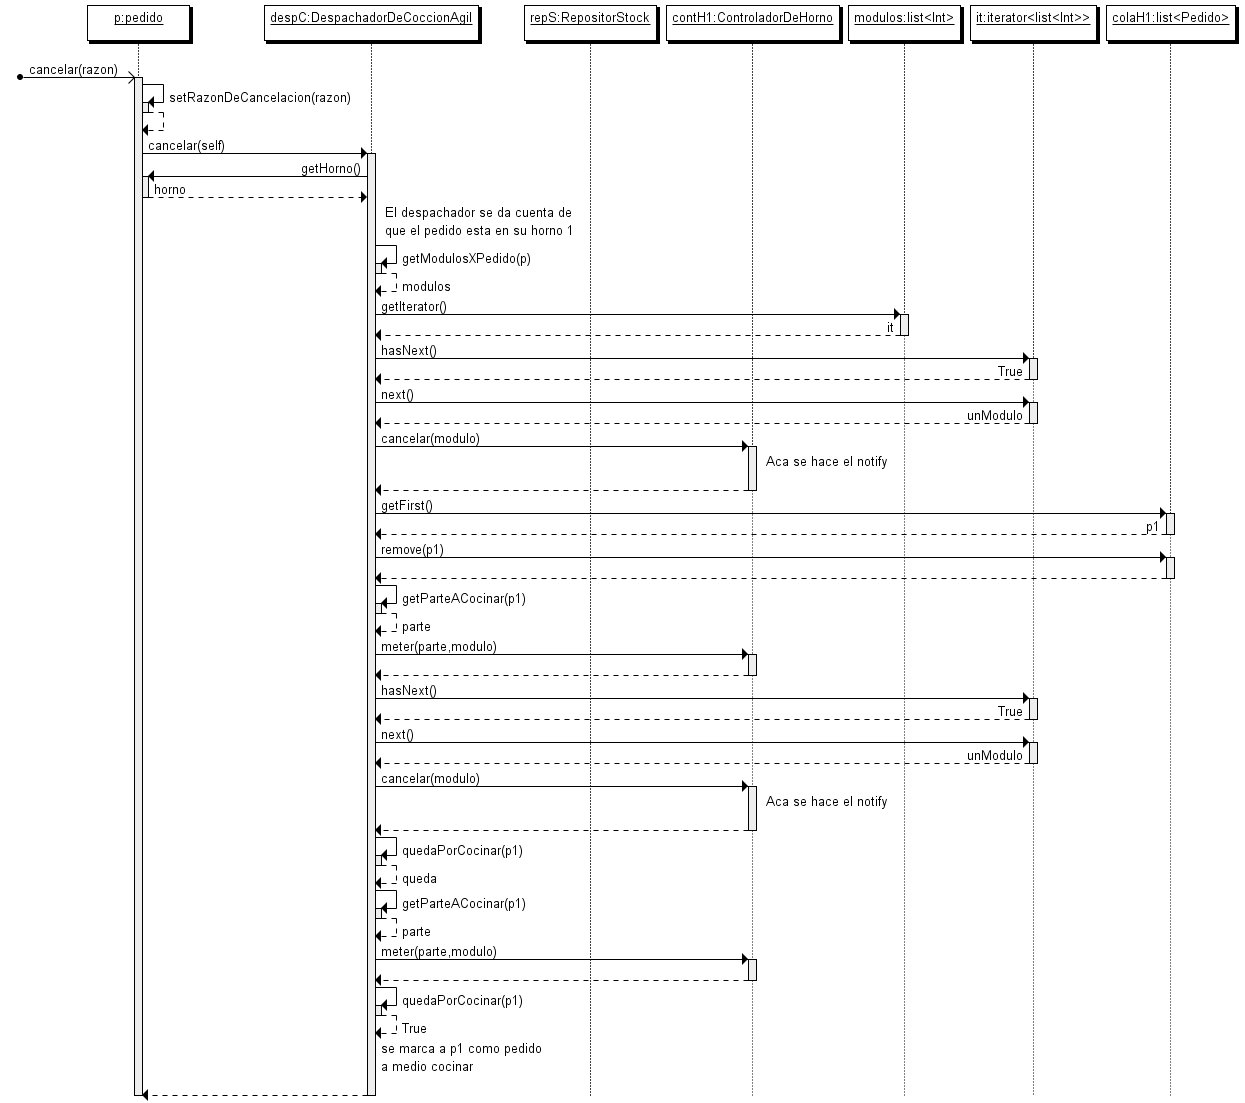
\includegraphics[height=19cm]{./figuras/cancelacionCoccion.png}
\caption{Cancelaci�n de un pedido en cocci�n}
\end{figure}

el m�todo getModulosPorPedido recorre el diccionario que guarda que pedido esta en cada m�dulo del horno del pedido para obtener en cuales se estaba cocinando el pedido, a fin de saber cuantos y cuales son los modulos que deben vaciarse y llenarse.

\begin{algorithm}[H]
\caption{Busca los modulos en los que se encuentra el pedido pe}
\begin{algorithmic}[1]
\PARAMS{p un pedido}
\STATE obtener la cantidad c de modulos del horno
\STATE modulo actual = primer modulo del horno de p
\WHILE{mientras hayan modulos por recorrer hacer}
\STATE obtener el pedido ped que se encuentra en el modulo i usando el diccionario
\IF{ped es p entonces}
\STATE agregar modulo actual en res
\ENDIF
\STATE modulo actual = siguiente modulo
\ENDWHILE
\RETURN res
\end{algorithmic}
\end{algorithm}

\subsubsection{Cancelaci�n de un pedido terminado}
En el caso de que se pretanda cancelar un pedido que esta en estado finalizado, se genera una excepcion. El escenario es simple, por lo que creemos que no es necesario un diagrama de secuencias.

\subsubsection{Otros escenarios}

La notificaci�n de cancelaci�n se propaga a la GUI que permite al maestro
reingresar insumos recuperables. Este evento es asincr�nico y la cancelaci�n
se concreta aunque el maestro no lleve a cabo la reposici�n, caso en el que
se asume que nada podr�a reponerse.

Se pueden seguir variando los par�metros pero la secuencia ser�a similar. 
Finalmente, la cancelaci�n tambi�n puede darse en el �mbito del controlador 
de entregas y del controlador de listos. En estos casos el manejo es simple, 
sin embargo, si el sistema dise�ado no correspondiente a la operaci�n de
contingencia podr�a existir una complejidad adicional producto de las notificaciones
al \textit{delivery}.

\subsubsection{Reponer el stock}
Cuando se produce una cancelaci�n, puede ser necesario reponer el stock, por ejemplo si el pedido estaba ingresado y no se utilizaron sus insumos. Como creiamos que hacer que el controlador maneje esta reposicion del stock no era adecuado (viola por ejemplo el principio de SRP, el controlador de ingreso solo se encarga de los pedidos ingresados, no tiene porque conocer los mecanismos de reposisici�n de stock). Por eso asociamos a la interfaz cancelador un repositor de stock.

El repositor de stock tiene la responsabilidad de devolver el stock cuando un pedido se cancela. Esto lo hace segun el estado del pedido, en particular si el pedido estaba preparandose, debe pedir que se ingresen los insumos salvables. 

Entonces consideremos el caso de un pedido ingresado. Al cancelarse todo su stock se puede reutilizar, de modo que la reposicion es completa. Veamos los siguientes diagramas de secuencias:

\begin{landscape}
\begin{figure}[H]
\centering
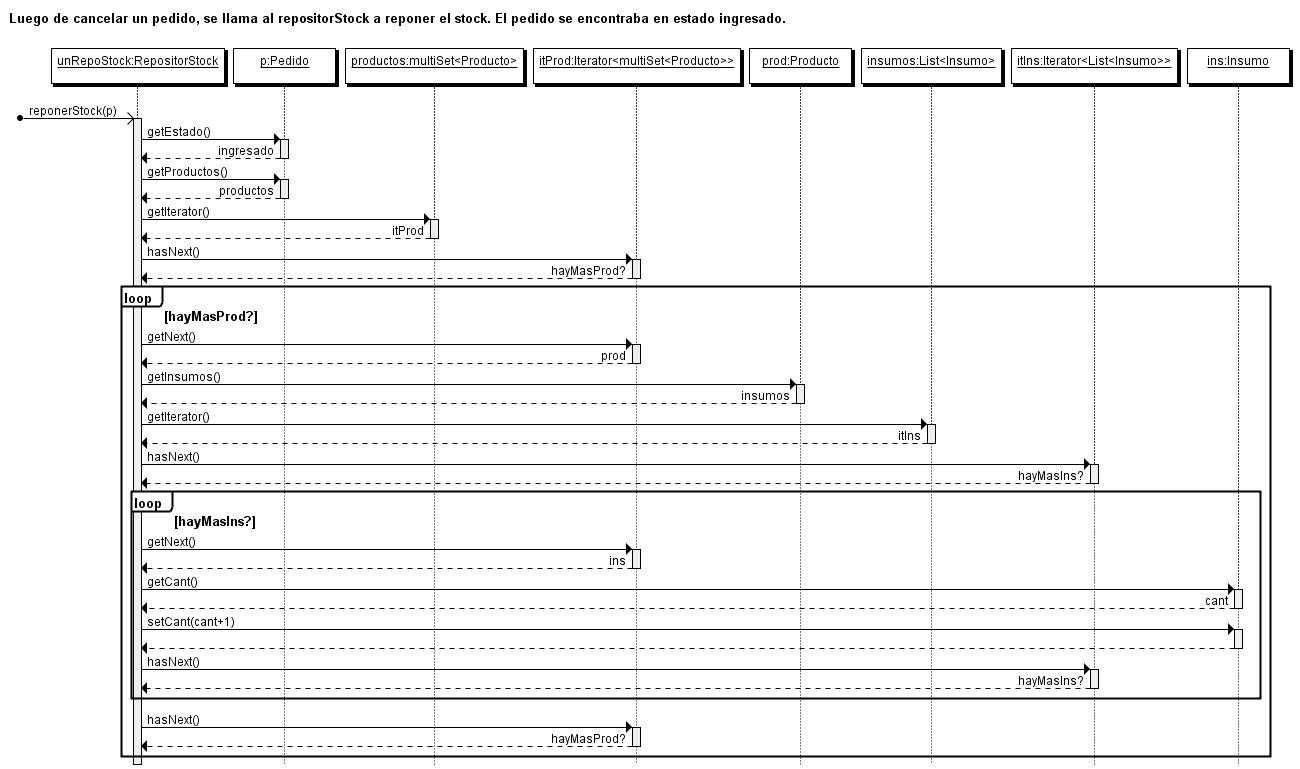
\includegraphics[height=16cm]{./figuras/repositorPedidoIngresado.png}
\caption{Reponer stock de pedido ingresado}
\end{figure}
\end{landscape}

\begin{landscape}
\begin{figure}[H]
\centering
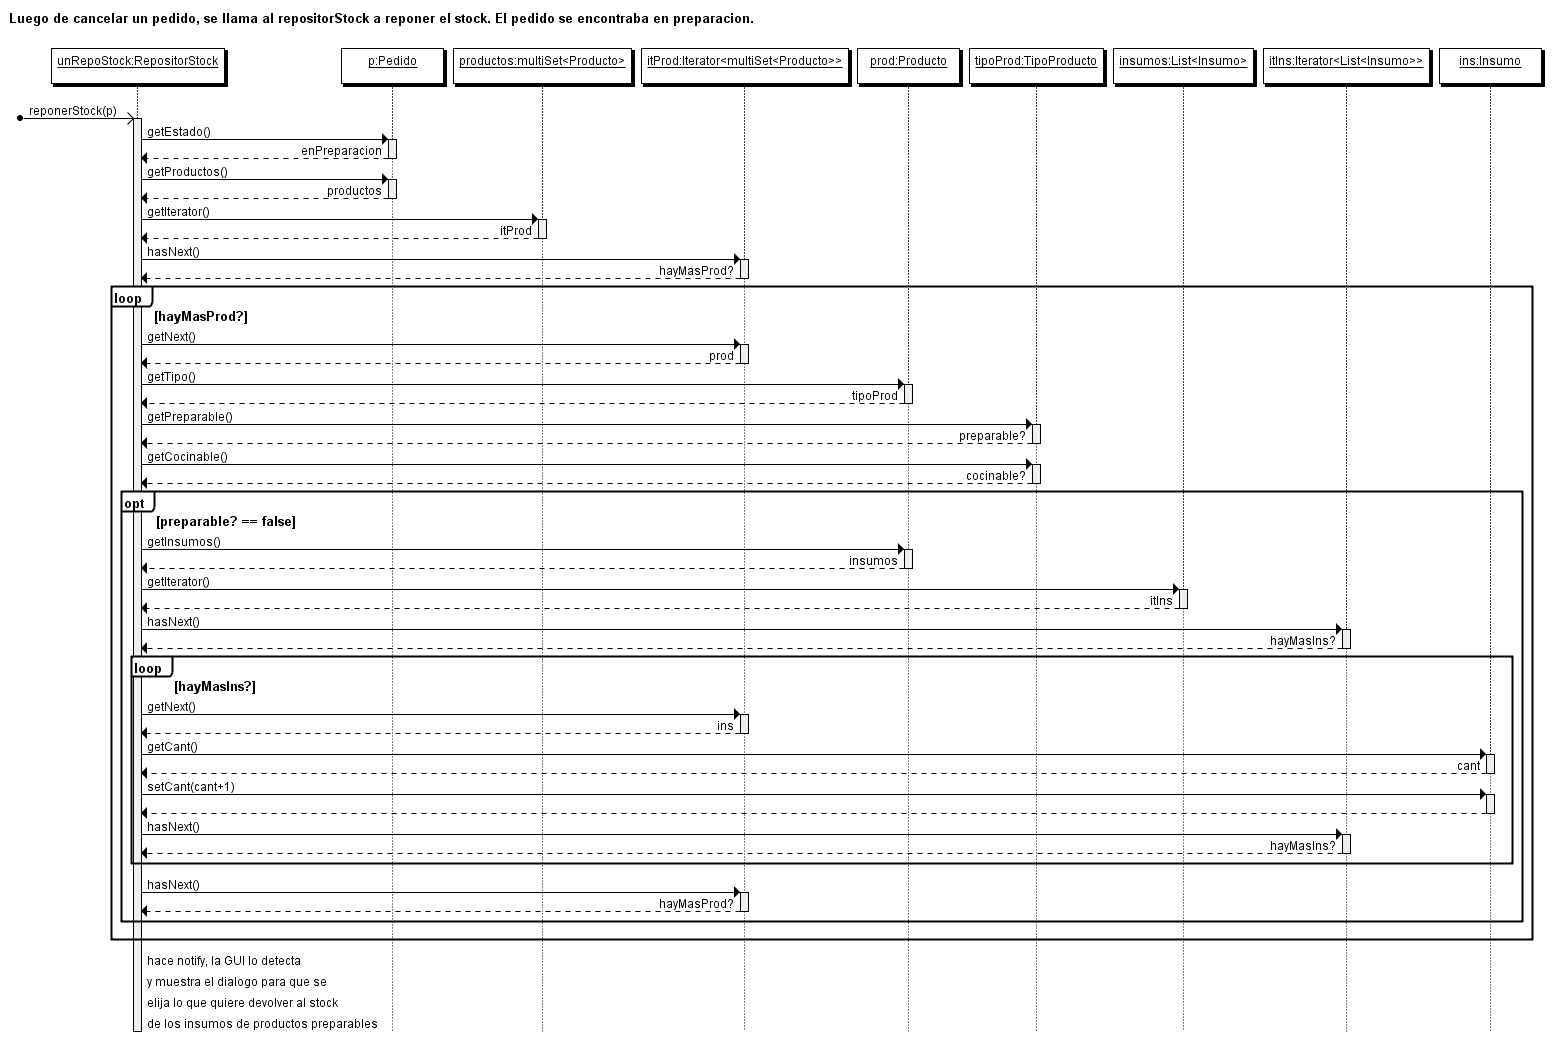
\includegraphics[height=16cm]{./figuras/repositorPedidoEnPreparacion.png}
\caption{Reponer stock de pedido en preparacion}
\end{figure}
\end{landscape}

\begin{landscape}
\begin{figure}[H]
\centering
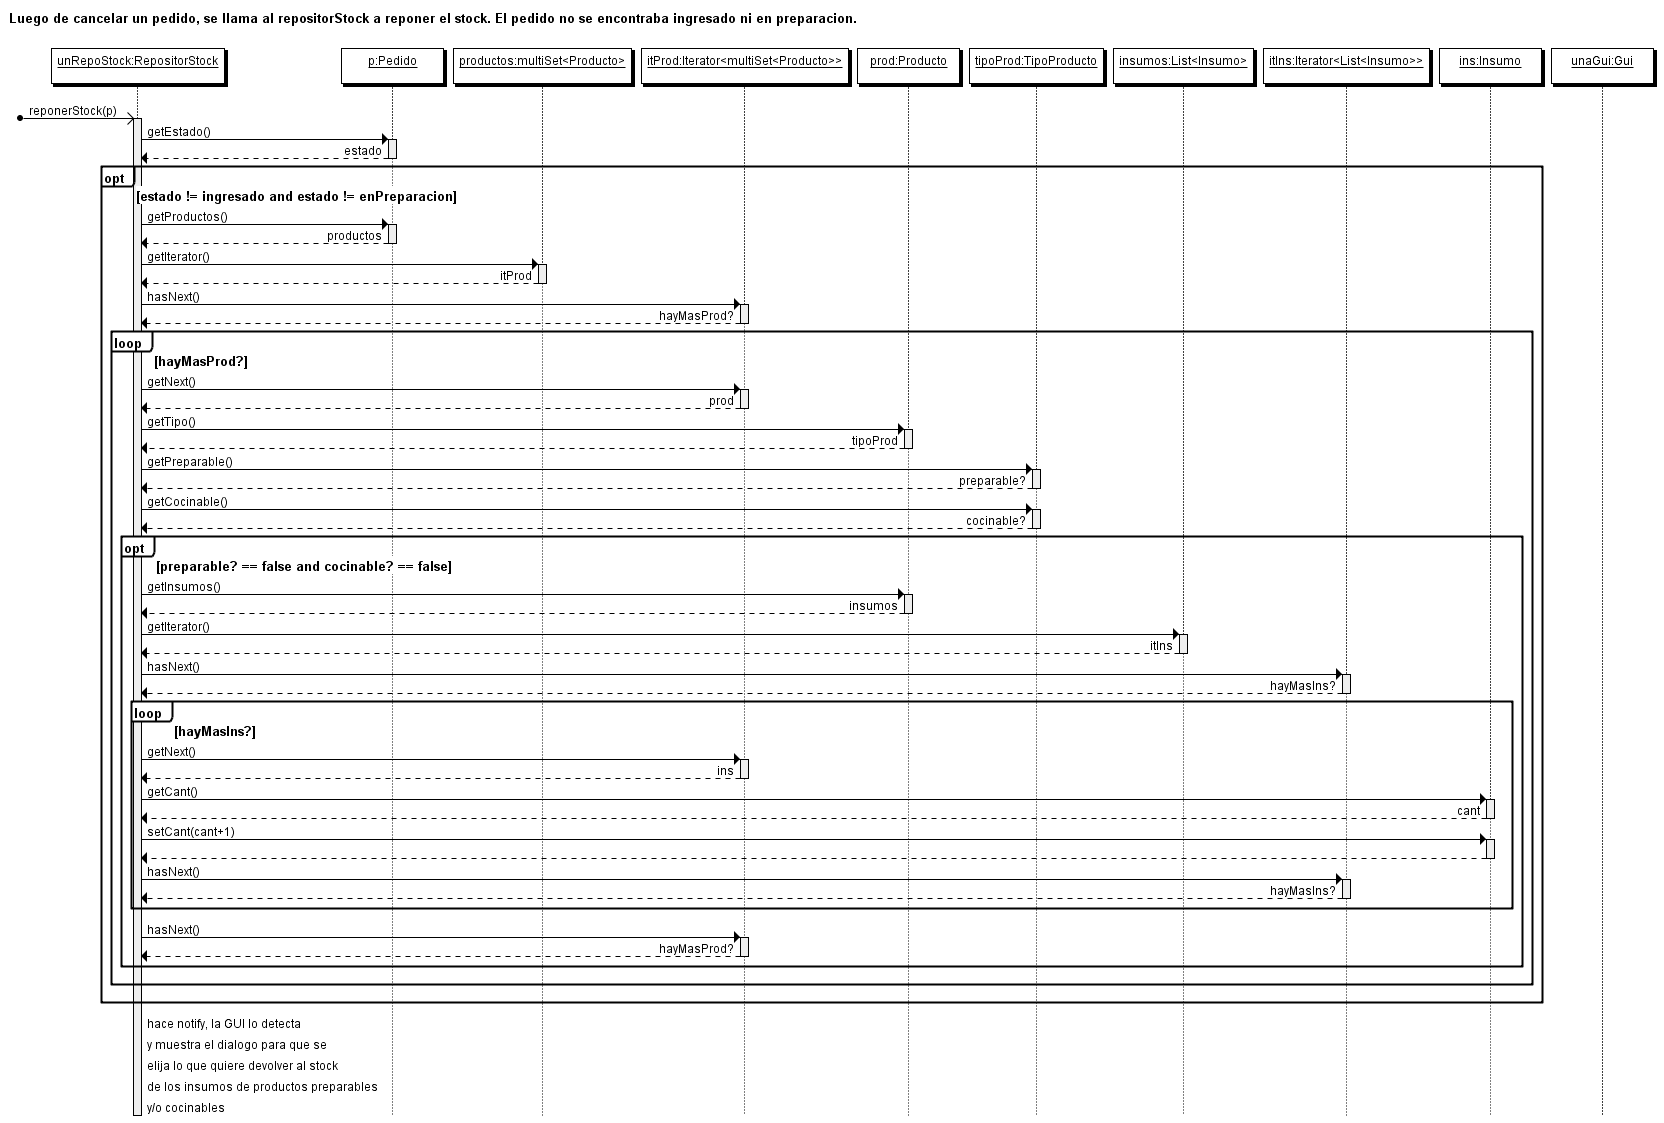
\includegraphics[height=15cm]{./figuras/repositorPedidoNoIngresadoNiPreparacion.png}
\caption{Reponer stock de pedidos en otro estado distinto}
\end{figure}
\end{landscape}

En el primer diagrama vemos que el estado sea ingresado y entonces procedemos a reponer todo el stock de sus productos.

Si el pedido se estaba preparando, hay que preguntar que hacer con los productos que son preparables, es decir pedir que insumos reponer y cuales ya fueron usados, esto se puede observar en el segundo diagrama.

Finalmente si el pedido ya esta totalmente preparado, la especificaci�n pide que solo se restablezca el stock de las bebidas. Eso es precisamente lo que se muestra en el �ltimo diagrama.

Notar que extendimos la especifiacion preguntando por los productos no preprables ni cocinables, de modo que por ejemplo si se venden por helados, al cancelar el pedido los helados se pueden reutilizar.


%
%\section{Explicación de las clases}
%\clase
%{ABMproductos}
%{Esta clase se encarga de realizar las altas, bajas y modificaciones de los productos}
%{}{}
%
%\clase
%{ABMstock}
%{Esta clase se encarga de realizar las altas, bajas y modificaciones de los insumos}
%{}{}
%
%\clase
%{Agil}
%{Especialización de gestor de horno, permite aplicar la politica agil}
%{}{}
%
%\clase
%{Aviso}
%{Clase utilizada para realizar el \textit{callback} desde el gestor de horno hacia el despachador de preparación, es la encargada de ejecutar el metodo del despachador que lo notifica de que se termino de preparar algo. Esta clase permite que el despachador no necesite saber quien le avisa, y por lo tanto permite que los preparadores no requieran de metodos diferenciados para avisar que se terminaron de preparar las pizzas, o las empanadas}
%{}{}
%
%\clase{Cliente}
%{Esta clase representa a un cliente, conteniendo todos los datos del mismo.}
%{}{}
%
%\clase{ColaListos} %FIXME: nombre poco feliz
%{Esta clase contiene a los pedidos que ya estan listos. Su responsabilidad es la de conocer a todos los que estan en este estado, a fin de que despachar un pedido se haga desde esta clase}
%{}{}
%
%\clase
%{ControladorDeIngreso}
%{Controla la cola de ingreso, la cual puede ser modificada por el encargado de pedidos. Cuando algun preparador queda libre, envia el proximo pedido a preparar}
%{}{}
%
%\clase
%{ControladorCliente}
%{El controlador de cliente tiene por responsabilidad encargarse de autentificar un usuario}
%{}{}
%
%\clase
%{ControladorStock}
%{El controlador de stock, tiene por responsabilidad chequear la disponibilidad de insumos al momento de un ingreso, asi como la de hacer el decremento del stock al ingresar un pedido, generando el aviso de stock critico en caso de ser necesario.}
%{}{}
%
%\clase
%{CoordinadorDePedidos}
%{El coordinador de pedidos se encarga de controlar el ingreso de pedidos, y su ciclo de vida fuera de la cocina}
%{}{}
%
%\clase
%{DespachadorDePreparación}
%{Esta clase tiene por responsabilidad manejar la cola de pedidos que se estan preparando, recordemos que puede existir una cola de preparaci'on si hay pedidos mixtos a la espera de uno de los maestros. El controlador de ingresos distribuye los pedidos a los distintos preparadores y despacha cada pedido a su gestor de horno correspondiente cuando ya esta preparado.}
%{}{}
%
%\clase
%{EstimadorDeTiempos}
%{El estimador de tiempos, como lo dice su nombre, se encarga de estimar el tiempo de preparacion y cocción de un pedido}
%{}{}
%
%\clase
%{GeneradorDePedidos}
%{Esta clase se encarga de crear pedidos, creando pedidos de solo bebidas o con comida segun los productos}%FIXME: justificacion
%{}{}
%
%\clase
%{GestorHorno}
%{Clase abstracta que permite implementar diferentes politicas para el manejo del horno}
%{}{}
%
%\clase
%{Insumo}
%{Contiene la información de los distintos insumos de la pizzería}
%{}{}
%
%\clase
%{Normal}
%{Permite implementar la politica normal de manejo del horno}
%{}{}
%
%\clase
%{Pedido}
%{Contiene la información de cada pedido}
%{}{}
%
